\chapter[Solução de Software]{Solução de Software}

\section{Arquitetura da Solução}

\subsection{Visão geral}

O escopo da solução de software envolve a implementação de uma interface \emph{Front End} e de microsserviços gerenciados por um \emph{API Gateway}. Envolve também a criação de módulos que ficarão instalados em componentes eletrônicos (\emph{Sistema Embarcado}). O objetivo da solução consiste em estabelecer a comunicação usuário - máquina através de um dispositivo móvel. Serão utilizados conceitos como Arquitetura de Microsserviços, \emph{Internet of Things}, \emph{Reactive Programming} e \emph{Cloud Deploy}. A figura abaixo representa uma visão ampliada da solução de software.

\begin{figure}[H]
    \centering
    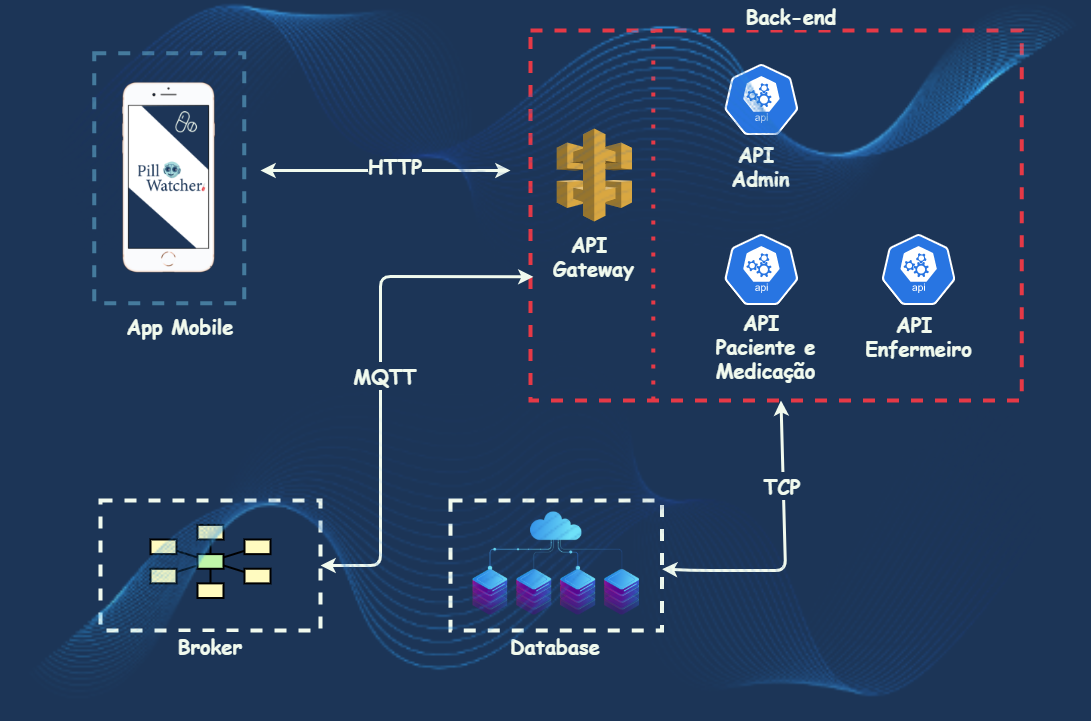
\includegraphics[width=1.0\textwidth]{figuras/solucao_software.png}
    \caption{Solução de Software}
    \label{fig:software_solution}
\end{figure}

\subsection{Banco de Dados}
Para armazenar dados referente à biometria, cadastro de pacientes, medicações, receitas e quaisquer tipo de conteúdos que se relacionam com a solução, optou-se pela utilização da tecnologia de banco de dados MySQL. 

O banco de dados relacional MySQL é um conjunto de dados relacionais, estruturados ou organizados na forma de tabelas, colunas e linhas, onde as tabelas representam os objetos, as colunas representam os campos e as linhas representam os registros \cite{EDUCBA_2020}.

Os dados referentes ao cadastro de medicações, pacientes, enfermeiros, entre outros, serão armazenados na nuvem, utilizando os servidores \textit{Linux} da \textit{One Click Hosting}. Por outro lado, dados referentes à biometria serão armazenados localmente, dentro da aplicação física, gerenciados pela \emph{Sistema Embarcado}.

O armazenamento na nuvem é adquirido de um fornecedor externo, que tem e opera capacidade de armazenamento físico de dados e entrega essa pela Internet com um modelo de pagamento conforme o uso. Esses fornecedores de armazenamento na nuvem gerenciam a capacidade, a segurança e a resiliência para disponibilizar dados aos aplicativos em todo o mundo \cite{AMAZONWEBSERVICES_2020}.

\subsection{Back-end}\label{sec:software_backend}
O \emph{Back-end} é a camada onde ocorre o processamento da lógica negocial. É o componente do software que estabelece conexão com a base de dados para registrar e/ou prover informações a um cliente. Tanto a aplicação móvel, quanto ao sistema embarcado instalado no dispensador de remédios se comunicarão com essa camada.

Será desenvolvido com a arquitetura de microsserviços, utilizando o \emph{framework} Spring (Boot, Data, Security) e \emph{libs} (bibliotecas) em \textit{Python} para a validação de impressões digitais. 
%e aplicação de aprendizado de máquina.
Tais aplicações estabelecerão comunicação entre si através de um sistema gerenciador (API Gateway), utilizando \textit{Spring Cloud}.

Também será responsável por fazer a integração com o dispensador de medicamentos, utilizando os conceitos de \emph{Internet of Things}. Para essa integração, será utilizado o \emph{middleware} de filas \textit{Mosquitto} para o repasse e recebimento de informações. As requisições à fila utilizam o protocolo MQTT.

A configuração de ambiente será realizada através da tecnologia \textit{Docker}. Em ambientes de produção, as aplicações serão implantadas nos servidores em nuvem da \textit{One Click Hosting}.

\subsection{Front-end}
A aplicação móvel, desenvolvida utilizando o \emph{framework} \textit{React Native}, proverá uma interface para o gerenciamento dos diversos tipos de usuários. Será responsável também por facilitar o gerenciamento de receitas médicas de seus pacientes e seus respectivos medicamentos, bem como notificar o enfermeiro(a) quando estiver no horário da medicação e quando o estoque de algum medicamento estiver baixo. A aplicação móvel tem como objetivo facilitar a análise de dados através da geração de gráficos e relatórios necessários aos seus usuários. 

Será responsável por validar medicamentos dispensados pela máquina e após esse procedimento, será exibida uma tela onde o profissional confirmará se a medicação foi ministrada ou não.


\subsection{Construção e Entrega de Software}
Para realizar a validação de alterações realizadas em código fonte, optou-se utilizar \textit{TravisCI} para integração contínua, onde são definidas as etapas descritas abaixo:

\begin{itemize}
    \item \emph{Build}: é construído o código-fonte e verificado se o mesmo está de acordo com padrões de Folha de Estilo pré-definidos;
    \item  \emph{Test}: são realizados os testes unitários e verificados se todos se encontram em estado aprovado;
    \item  \emph{SonarQube Analysis}: o código-fonte é analisado e comparado com métricas de Confiabilidade, Segurança, Manutenibilidade, Cobertura de Testes e Duplicação de Código;
    \item  \emph{Deploy}: a solução é implantada em um ambiente de produção e/ou desenvolvimento. 
\end{itemize}

O\textit{SonarQube} conforme descrito acima na etapa de \textit{SonarQube Analysis}, trata-se de uma ferramenta em código aberto desenvolvida pela empresa \textit{SonarSource} para inspeção contínua da qualidade do código, execução de revisões automáticas com análise estática do código para detecção de odores de código e vulnerabilidades de segurança em mais de 20 linguagens de programação. Com o objetivo de entregar um código testado e livre de inconsistências, optou-se pela utilização do conceito TDD (\emph{Test Driven Development}), o qual consiste no desenvolvimento de testes unitários antes do desenvolvimento de funcionalidades. Optou-se também pela metodologia de desenvolvimento orientado à métricas (os quais o SonarQube mede e valida).

\begin{figure}[H]
    \centering
    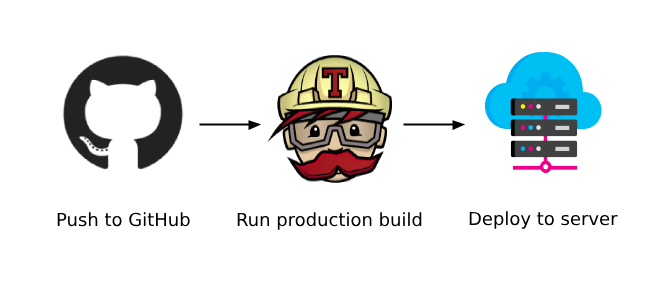
\includegraphics[width=1.0\textwidth]{figuras/deploy-continuous.png}
    \caption{Software Deploy}
    \label{fig:software_deploy}
\end{figure}

A etapa de \emph{Deploy}, listada acima, depende que haja um ambiente pré configurado para ser realizada. Para isso, optou-se utilizar \textit{Docker} para conteinerização de softwares auxiliares e a \textit{One Click Hosting} para hospedagem dos serviços em nuvem.

\section{Arquitetura da Informação}

\subsection{Modelo Entidade Relacionamento - MER}

O Modelo Entidade Relacionamento (também chamado Modelo ER, ou simplesmente MER), como o nome sugere, é um modelo conceitual utilizado na Engenharia de Software para descrever os objetos (entidades) envolvidos em um domínio de negócios, com suas características (atributos) e como elas se relacionam entre si (relacionamentos).\cite{DEVMEDIA_2014}

O MER abaixo representa as entidades necessárias para desenvolver o aplicativo PillWatcher. Fora utilizado o idioma Inglês para descrever as entidades e seus atributos. A modelagem está na quarta forma normal, assim atendendo as principais regras de qualidade de banco de dados.

\begin{figure}[H]
    \centering
    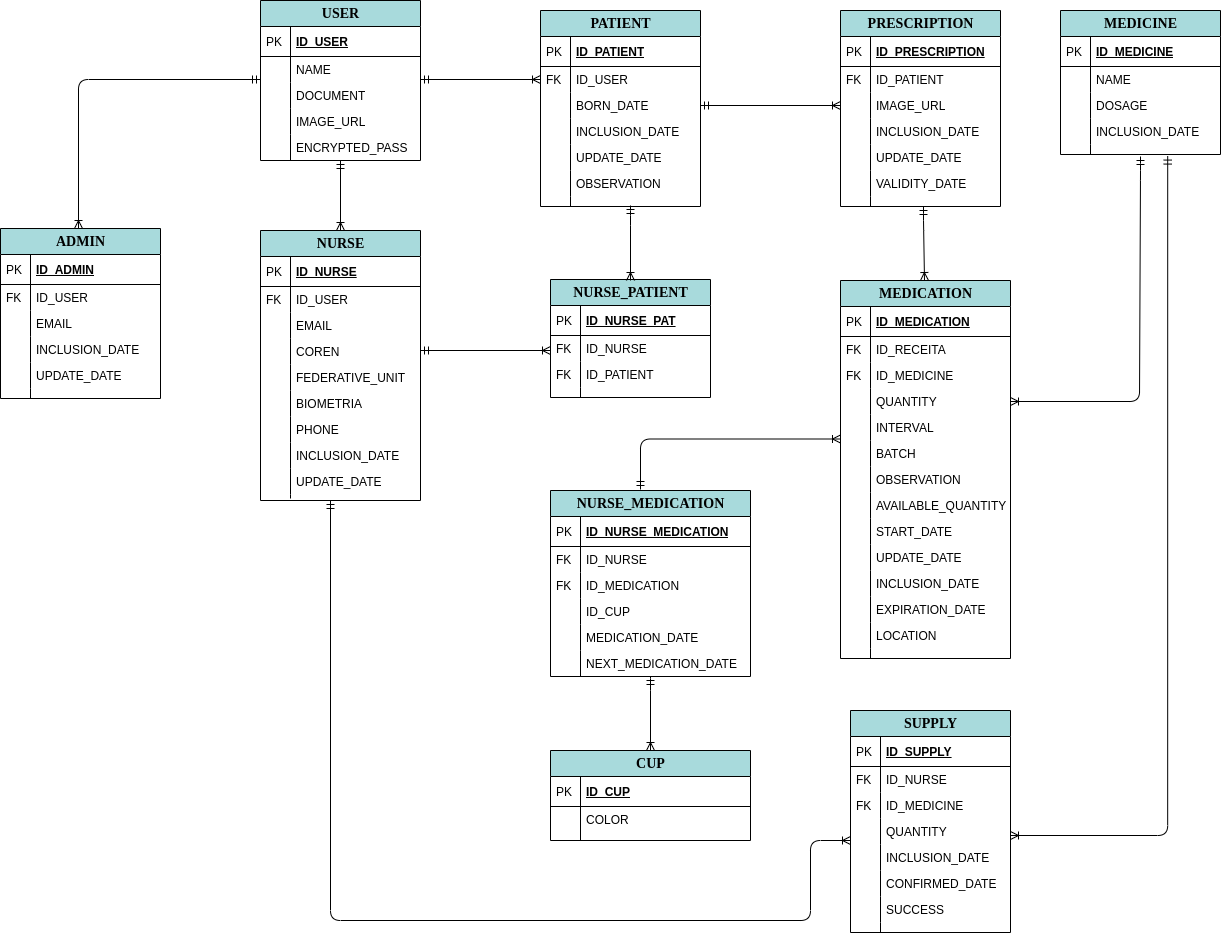
\includegraphics[width=0.9\textwidth]{figuras/database.png}
    \caption{MER}
    \label{fig:der}
\end{figure}

Para melhor entendimento, seguem breves explicações de cada entidade:

\begin{enumerate}
  \item USER: um usuário generalizado.
  \item ADMIN: especialização de User, representa o administrador do sistema.
  \item NURSE: especialização de User, representa o enfermeiro do sistema.
  \item PATIENT: especialização de User, representa o paciente do sistema.
  \item NURSE PATIENT: associação entre paciente e enfermeiro. Pois um enfermeiro pode cuidar de vários pacientes, e um paciente pode ser observado por vários enfermeiros.
  \item PRESCRIPTION: receita médica de um paciente.
  \item MEDICATION: medicação que compõe uma receita.
  \item NURSE MEDICATION: associação entre enfermeiro e medicação. Pois uma medicação ao paciente é gerida por um enfermeiro.
  \item CUP: copo para medicação ao paciente.
  \item SUPPLY: abastecimento feito no dispensador por um enfermeiro.
  \item MEDICINE: remédio disponível no dispensador e que compõe uma medicação.
\end{enumerate}

\section{Diagramas UML}

Os diagramas UML podem ajudar arquitetos e desenvolvedores de sistema a entender, colaborar e desenvolver um aplicativo. Arquitetos e gerenciadores de alto nível podem usar diagramas UML para visualizar todo o sistema ou projeto e separar aplicativos em componentes menores para desenvolvimento.\cite{IBM}

Existem diferentes tipos de diagramas UML, e para o projeto foram escolhidos os de caso de uso, pacotes e sequência. Juntos, eles trazem uma visão dos requisitos do sistema, arquitetura interna do back-end e também uma visão geral das atividades.

\section{Diagramas de Caso de Uso}

Os diagramas de casos de uso descrevem as funções principais de um sistema e identificam as interações entre o sistema e seu ambiente externo, representado por agentes. Esses agentes podem ser pessoas, organizações, máquinas ou outros sistemas externos\cite{IBM}. Abaixo tem os diagramas separados dos principais usuários do sistema.

\begin{enumerate}
    \item Diagrama de Caso de Uso do Mantenedor
    
\begin{figure}[H]
    \centering
    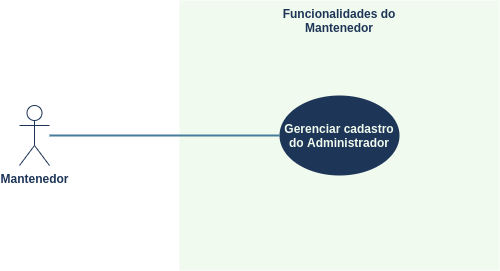
\includegraphics[width=0.5\textwidth]{figuras/matenedor-us.png}
    \caption{Caso de Uso - Mantenedor}
    \label{fig:mantenedor_us}
\end{figure}

Nesse diagrama, foi listada a principal e única funcionalidade do usuário mantenedor.
    \item Diagrama de Caso de Uso do Sistema
    
\begin{figure}[H]
    \centering
    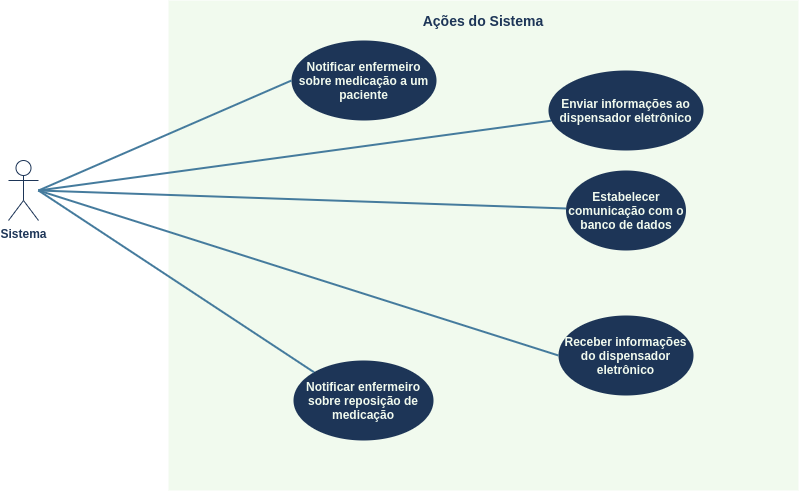
\includegraphics[width=0.5\textwidth]{figuras/sistema-us.png}
    \caption{Caso de Uso - Sistema}
    \label{fig:sistema_us}
\end{figure}

Nesse digrama foram listadas as principais ações do sistema. O Diagrama de Caso de Uso executa diversas ações isoladamente que são de extrema importância para o fluxo do projeto PillWatcher, como notificar o enfermeiro de ações que ele deve tomar.

    \item Diagrama de Caso de Uso do Enfermeiro
    
\begin{figure}[H]
    \centering
    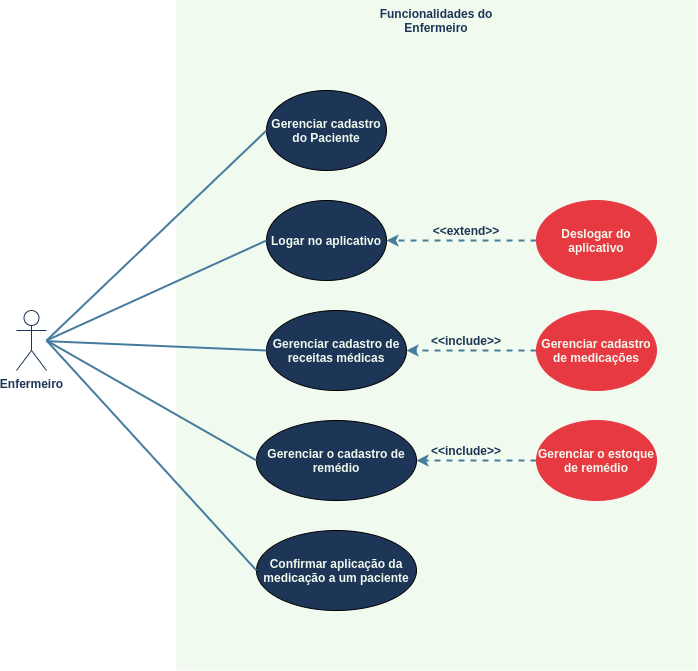
\includegraphics[width=0.5\textwidth]{figuras/enfermeiro-us.png}
    \caption{Caso de Uso - Enfermeiro}
    \label{fig:enfermeiro_us}
\end{figure}

Nesse digrama, foram listadas as principais funcionalidades do enfermeiro. Esse é o usuário principal do sistema.

    \item Diagrama de Caso de Uso do Administrador

\begin{figure}[H]
    \centering
    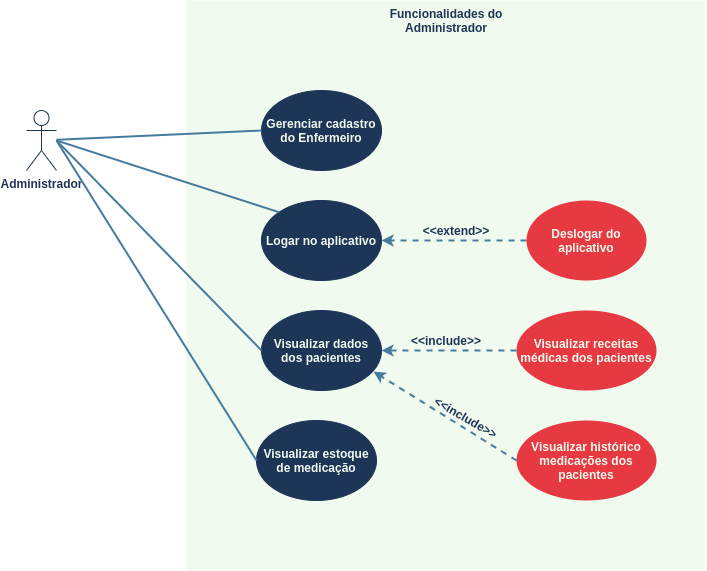
\includegraphics[width=0.6\textwidth]{figuras/administrador-us.png}
    \caption{Caso de Uso - Administrador}
    \label{fig:administrador_us}
\end{figure}

Nesse digrama, foram listadas as principais funcionalidades do administrador. Esse usuário apenas gerencia o cadastro do enfermeiro e visualiza todos os dados disponíveis no aplicativo.

\end{enumerate}

\section{Diagrama de Pacotes}

Diagramas de pacotes são módulos do sistema divididos em agrupamentos lógicos mostrando a dependência entre eles.
Foi diagramado os pacotes que fazem parte da solução back-end, como mostra a imagem \ref{fig:pacotes-diagrama}. Assim, cada pacote ilustrado tem um papel específico dentro do projeto, e estão descritos abaixo:

\begin{enumerate}
  \item Controllers: possui todas as classes que se comunicam com o mundo externo por meio de requisições HTTP.
  \item Constants: possui classes/interfaces com atributos contantes utilizados em todo o projeto.
  \item Services: possui classes/interfaces que implementam a lógica negocial.
  \item Mappers: possui interfaces que tranformam um objeto em outro.
  \item Repositories: possui interfaces que se comunicam com o banco de dados.
  \item Entities: possui classes que são representação de entidades no banco de dados.
  \item Utils: possui classes utilitárias, usadas por todo o projeto.
  \item Exceptions: possui classes que definem todas as exceções geradas no projeto.
  \item Handler: possui classes que tratam as exceções geradas no projeto.
\end{enumerate}

\begin{figure}[H]
    \centering
    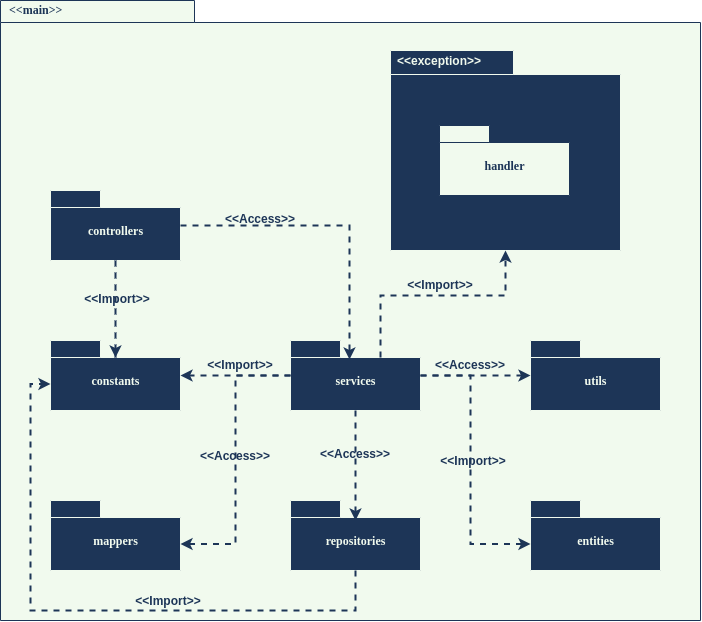
\includegraphics[width=0.9\textwidth]{figuras/diagrama-pacote.png}
    \caption{Diagrama de Pacotes do Back-end}
    \label{fig:pacotes-diagrama}
\end{figure}



\section{Nonfunctional Requirements (NFRs) }

Os Requisitos Não Funcionais (NFRs) definem os atributos do sistema, como segurança, confiabilidade, desempenho, escalabilidade e usabilidade. Eles servem como restrições ou restrições ao design do sistema entre os diferentes acúmulos.

Também conhecidos como qualidades do sistema, os requisitos não funcionais são tão críticos quanto as epopeias, recursos e histórias funcionais . Eles garantem a usabilidade e eficácia de todo o sistema. O não cumprimento de qualquer um deles pode resultar em sistemas que não atendem às necessidades internas do negócio, do usuário ou do mercado.

Um aspecto importante em uma solução de software é a confiabilidade representada na figura \ref{fig:nfr-confiabilidade}. Para atingir essa meta, foram levantadas 3 condições que precisam ser atendidas para essa característica ser cumprida, são elas: proteção de dados dos usuários, autenticação de contas e limitação no cadastro. Para alcançar a primeira, será utilizada a tecnologia \textit{Spring Security} que assegurará os dados dos usuários. A segunda será satisfeita por meio da utilização de biometria e de login por CPF e senha. Por último, a solução atua em um cenário sensível, assim é necessário garantir uma limitação no cadastro que será totalizada quando o administrador for inserido na aplicação, esse irá cadastrar os enfermeiros, os quais, por conseguinte, serão os responsáveis pelo cadastro dos pacientes e dos familiares. 

\begin{figure}[H]
    \centering
    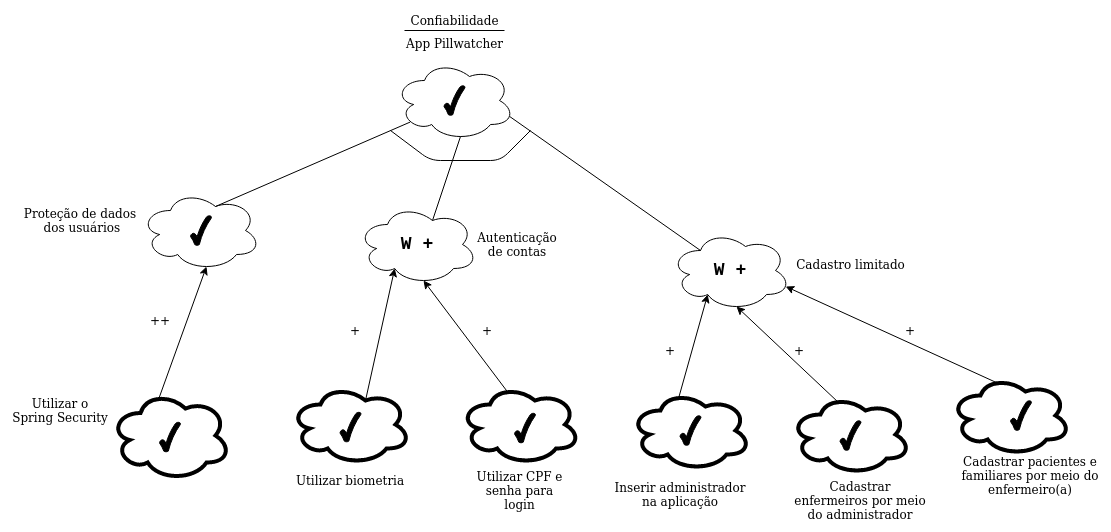
\includegraphics[width=0.7\textwidth]{figuras/NFR_Confiabilidade.png}
    \caption{NFR de confiabilidade}
    \label{fig:nfr-confiabilidade}
\end{figure}

Outro aspecto extremamente importante para o desenvolvimento de um software seguro é assegurar que os pilares (Autenticidade, Confidencialidade e Integridade) estejam presentes conforme apresentado na figura \ref{fig:nfr-seguranca}. Para garantir a autenticidade do sistema será implementado um sistema de autenticação de dados do usuário que poderá ter acesso à aplicação. Para que o pilar da Confidencialidade seja satisfeito, será aplicado ao sistema o gerenciamento de acessos que dará permissões restritas a depender do tipo de usuário cadastrado. O pilar de integridade do sistema fica por conta da verificação e execução dos testes de software como por exemplo os testes unitários.

\begin{figure}[H]
    \centering
    \includegraphics[width=0.6\textwidth]{figuras/nfr_segurança.png}
    \caption{NFR de segurança}
    \label{fig:nfr-seguranca}
\end{figure}

Com relação aos aspectos relevantes que afetam o desempenho da aplicação, temos o a redução do uso de memória por meio de uma dinâmica de páginas que reduzam o volume de informações apresentadas diretamente em tela, a melhoria do design será garantido por meio da aplicação de um design minimalista e a redução da utilização de recursos do servidor e otimização do tempo de resposta se darão por meio da hospedagem de um servidor eficiente como o Heroku.

\begin{figure}[H]
    \centering
    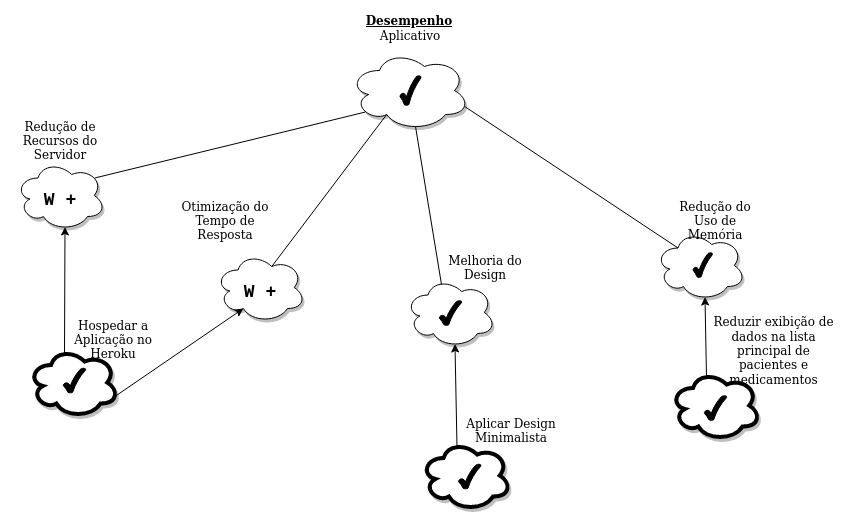
\includegraphics[width=0.7\textwidth]{figuras/NFR_Desempenho.png}
    \caption{NFR de desempenho}
    \label{fig:nfr-desempenho}
\end{figure}

Para atender aos módulos de usabilidade da aplicação e consequentemente atender as necessidades de utilização do usuário, estaremos dando enfoque em três pontos principais: Boa comunicação, por meio da utilização de mensagens significativas e de boa compreensão do usuário,implementação de uma interface simples por meio de uma boa organização de elementos, bem como a consistência e padronização dos componentes. Outro ponto é a facilidade de utilização que exija uma curva de aprendizado menor do usuário em relação a utilização da aplicação por meio de um design intuitivo.
\begin{figure}[H]
    \centering
    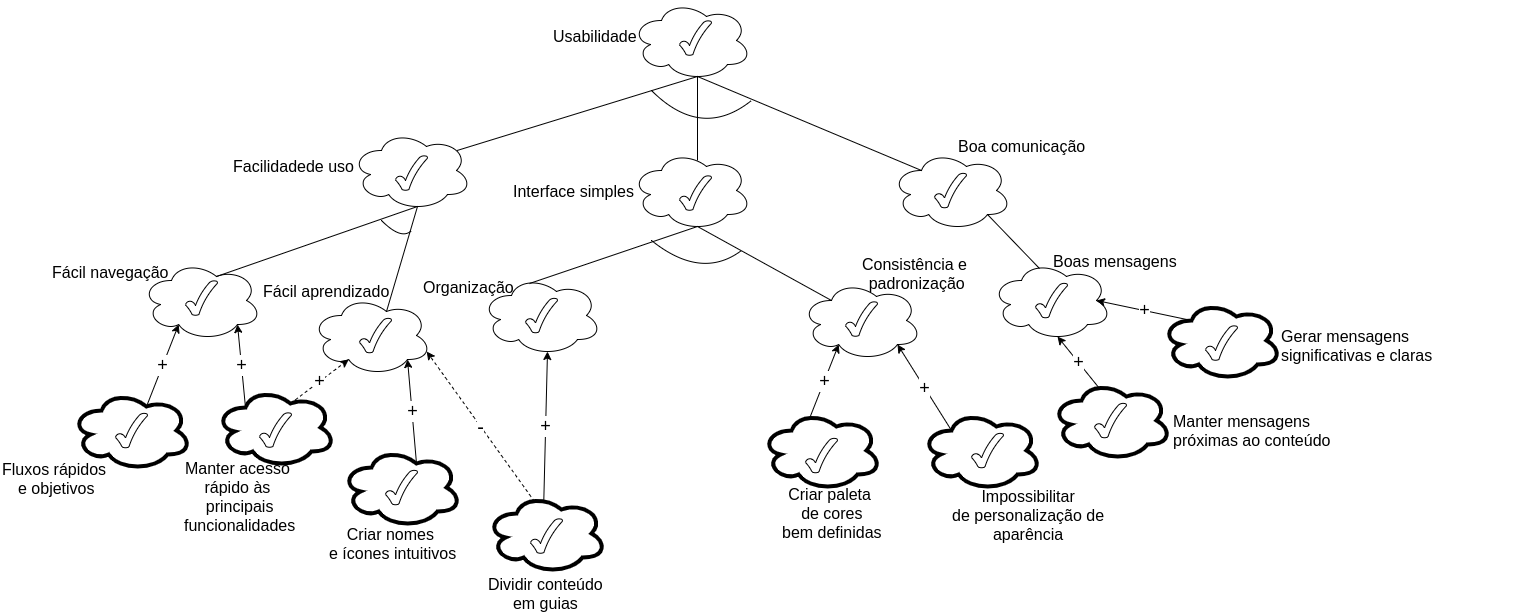
\includegraphics[width=0.9\textwidth]{figuras/nfr_usabilidade_pill.png}
    \caption{NFR de usabilidade}
    \label{fig:nfr-usabilidade}
\end{figure}

\section{Inovação no Software}
\subsection {IoT - Internet of Things}
\textit{Internet of Things} é a interconexão de objetos com a internet. No projeto PillWatcher, o dispensador de medicamentos irá se comunicar com o aplicativo por meio de um \textit{Broker} MQTT, que é como uma espécie de mediador entre as máquinas, capaz de fazer com que a comunicação de fato ocorra entre elas. O \textit{Broker} utilizado será o \textit{Mosquitto}.

O protocolo MQTT é um dos mais utilizados na indústria para a implementação de automações e de tecnologias como a IoT – internet das coisas. Sigla para \textit{Message Queuing Telemetry Transporte}, ele pode ser resumido como uma forma de realizar a comunicação entre as máquinas.\cite{ENGPROCESS_2018}

E o \textit{Mosquitto} nada mais é do que um dos componentes do protocolos MQTT. Cada vez mais usado no setor industrial, ele aparece como uma forma de otimizar o tempo e tornar os processos mais simples \cite{ENGPROCESS_2018}.

\subsection {Arquitetura de Microsserviços}
A arquitetura de microsserviços permite a entrega e implantação contínua de aplicações grandes e complexas. Além disso, há a melhoria na manutenção, onde cada serviço é relativamente pequeno e, portanto, mais fácil de entender e mudar. Traz consigo também uma melhor testabilidade, devido ao fato de que os serviços são menores e mais rápidos de testar. A implantabilidade dos serviços podem ser feitas de forma independente e permite que a organização do esforço de desenvolvimento em torno de várias equipes seja autônoma.

\subsection {Reactive Programming}
A programação reativa é um paradigma de programação assíncrona, preocupado com fluxos de dados e a propagação de mudanças. Isso significa que é possível expressar fluxos de dados estáticos (por exemplo, matrizes) ou dinâmicos (por exemplo, emissores de eventos com facilidade por meio da  linguagem  de programação empregada. 

\section{Protótipo de Alta Fidelidade}
A prototipagem de alta fidelidade é a técnica que mais se aproxima do produto final. Por meio da aplicação dessa, é possível avaliar questões de Interface do Usuário (UI -  User Interface) e de Experiência do Usuário \textit{(UX - User Experience)}. Sendo esses conteúdos extremamente relevantes em termos de desenvolvimento de \textit{front-end}. Abaixo está ilustrado o protótipo desenvolvido para o Pillwatcher divido por fluxo de cada perfil de usuário.  

\subsection{Login}

A tela \ref{fig:prototipo_tela_inicial_e_login} será exibida logo após a inicialização da aplicação móvel. A tela de login será responsável por autenticar os usuários via CPF e senha e por oferecer a opção de recuperação de senha, caso o usuário a tenha esquecido. A figura \ref{fig:prototipo_fluxo_recuperar_senha} retrata o fluxo de recuperação de senha. Caso essa opção tenha sido selecionada, o próprio digitará o email cadastrado na terceira tela e receberá um \textit{feedback} dessa ação na quarta tela.

\begin{figure}[H]
    \centering
    \subfloat[][Tela inicial e tela de login]{
    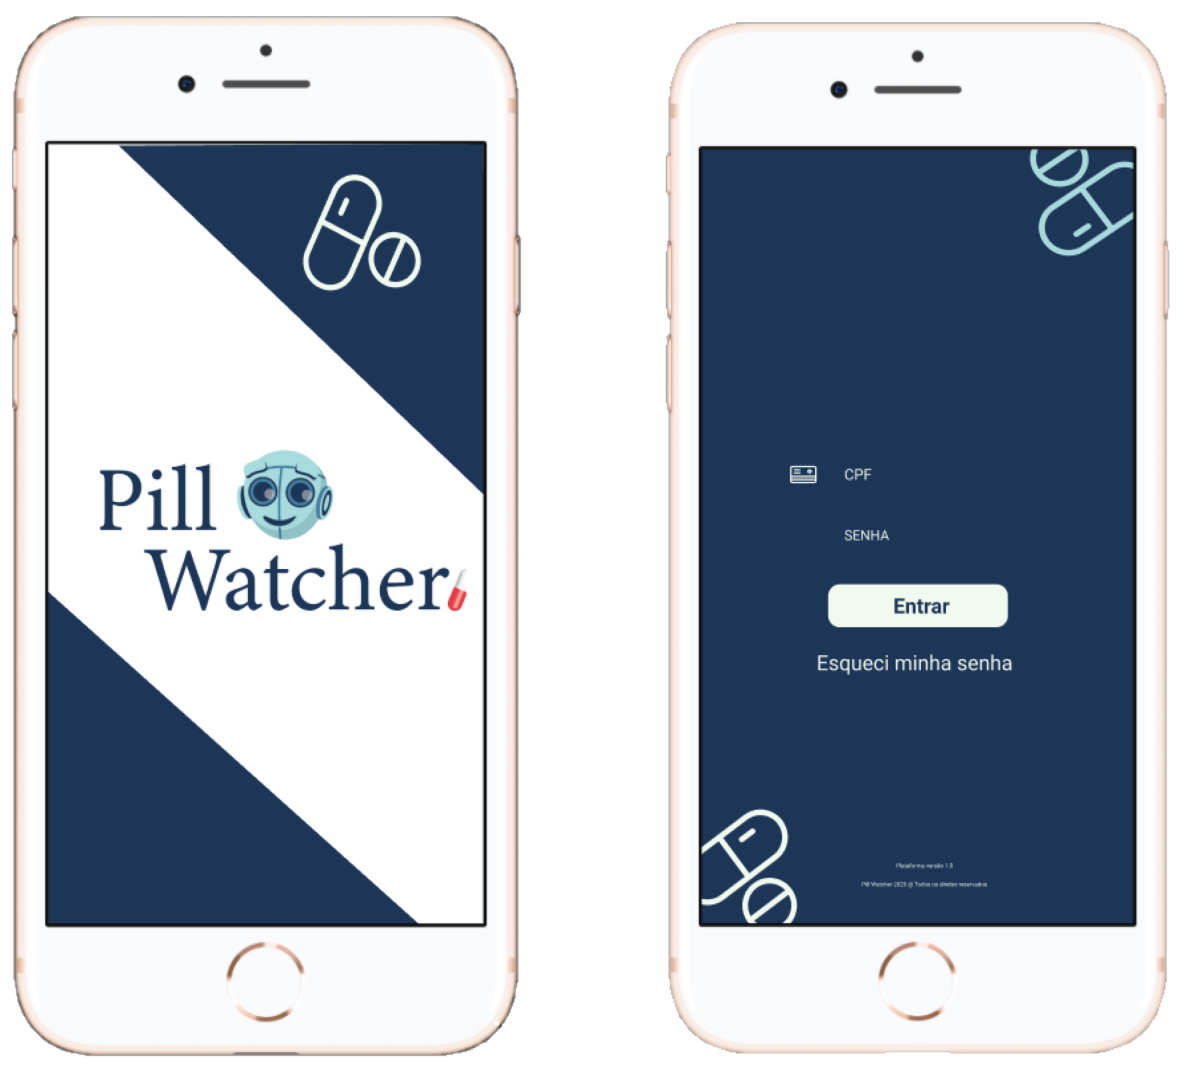
\includegraphics[width=8cm]{figuras/Software_Prototipo/Prototipo_Fluxo_Login_1.png}
    \label{fig:prototipo_tela_inicial_e_login}}
\end{figure}
    
\begin{figure}[H]
    \centering
    \subfloat[][Fluxo para recuperar senha]{
    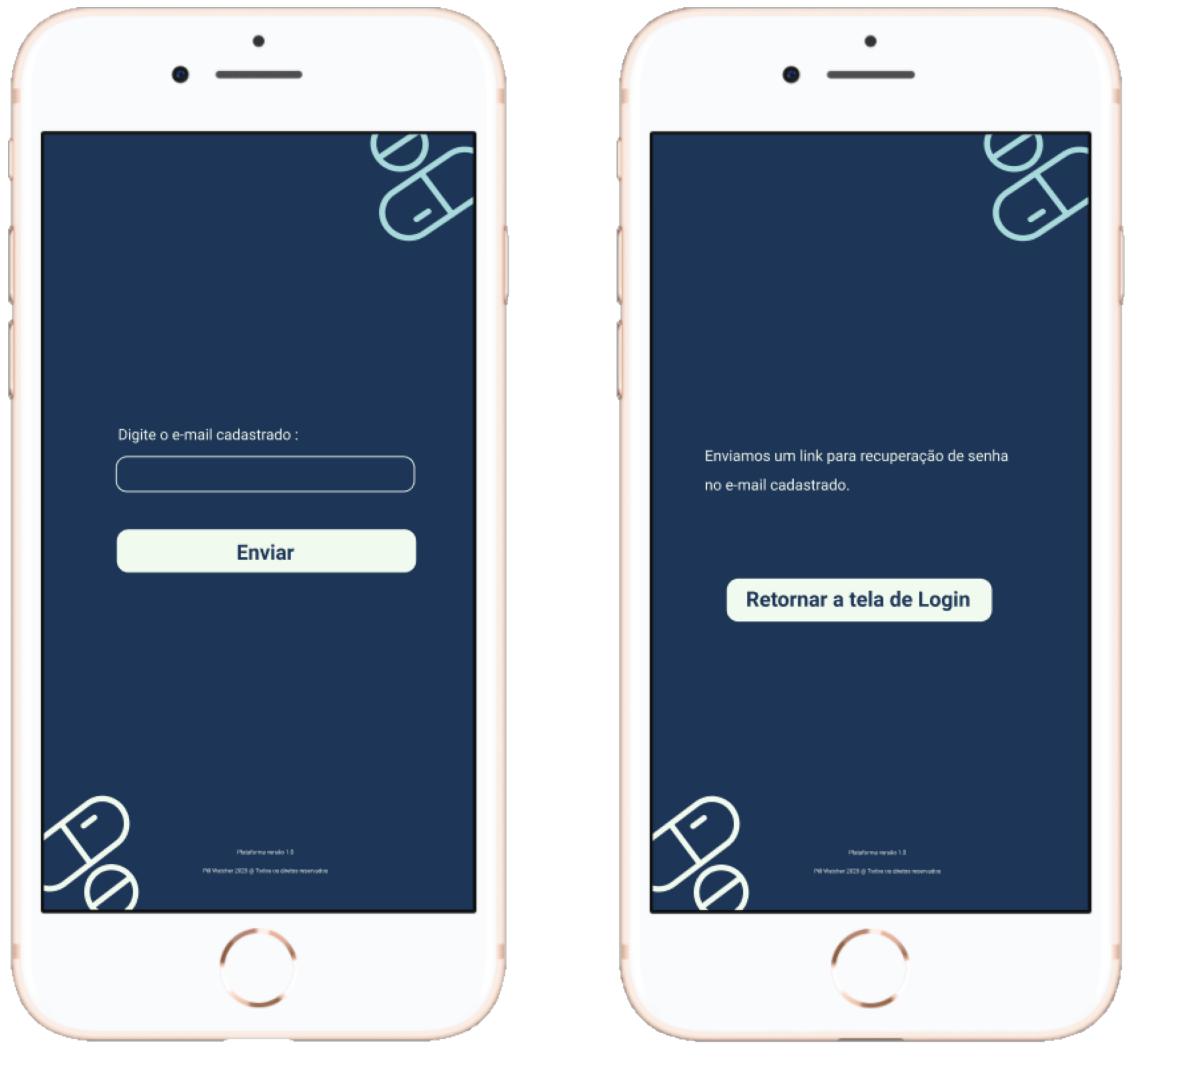
\includegraphics[width=8cm]{figuras/Software_Prototipo/Prototipo_Fluxo_Login_2.png}
    \label{fig:prototipo_fluxo_recuperar_senha}}
    \caption{Fluxo de Login}
\end{figure}

 
\subsection{Administrador(a)}
\begin{figure}[H]
    \centering
    \subfloat[][Sidebar e tela para alterar dados do perfil]{
    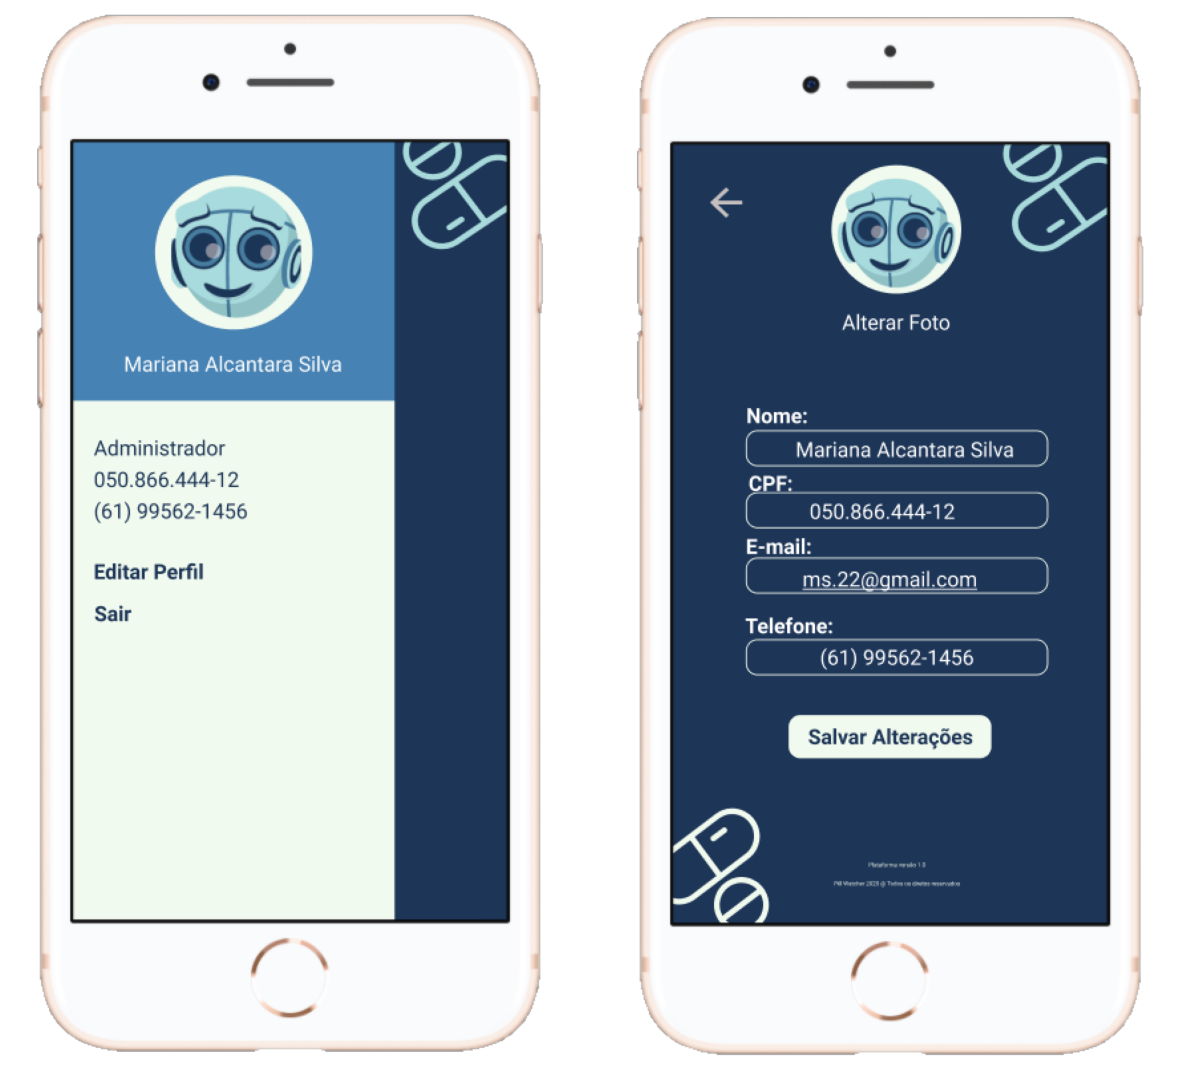
\includegraphics[width=8cm]{figuras/Software_Prototipo/Prototipo_Fluxo_Administrador_1.png}
    \label{fig:prototipo_sidebar_e_alterar_dados}}
\end{figure}
    
\begin{figure}[H]
    \centering
    \subfloat[][Menu Inicial e Etapa 1 do cadastro de enfermeiro(a)]{
    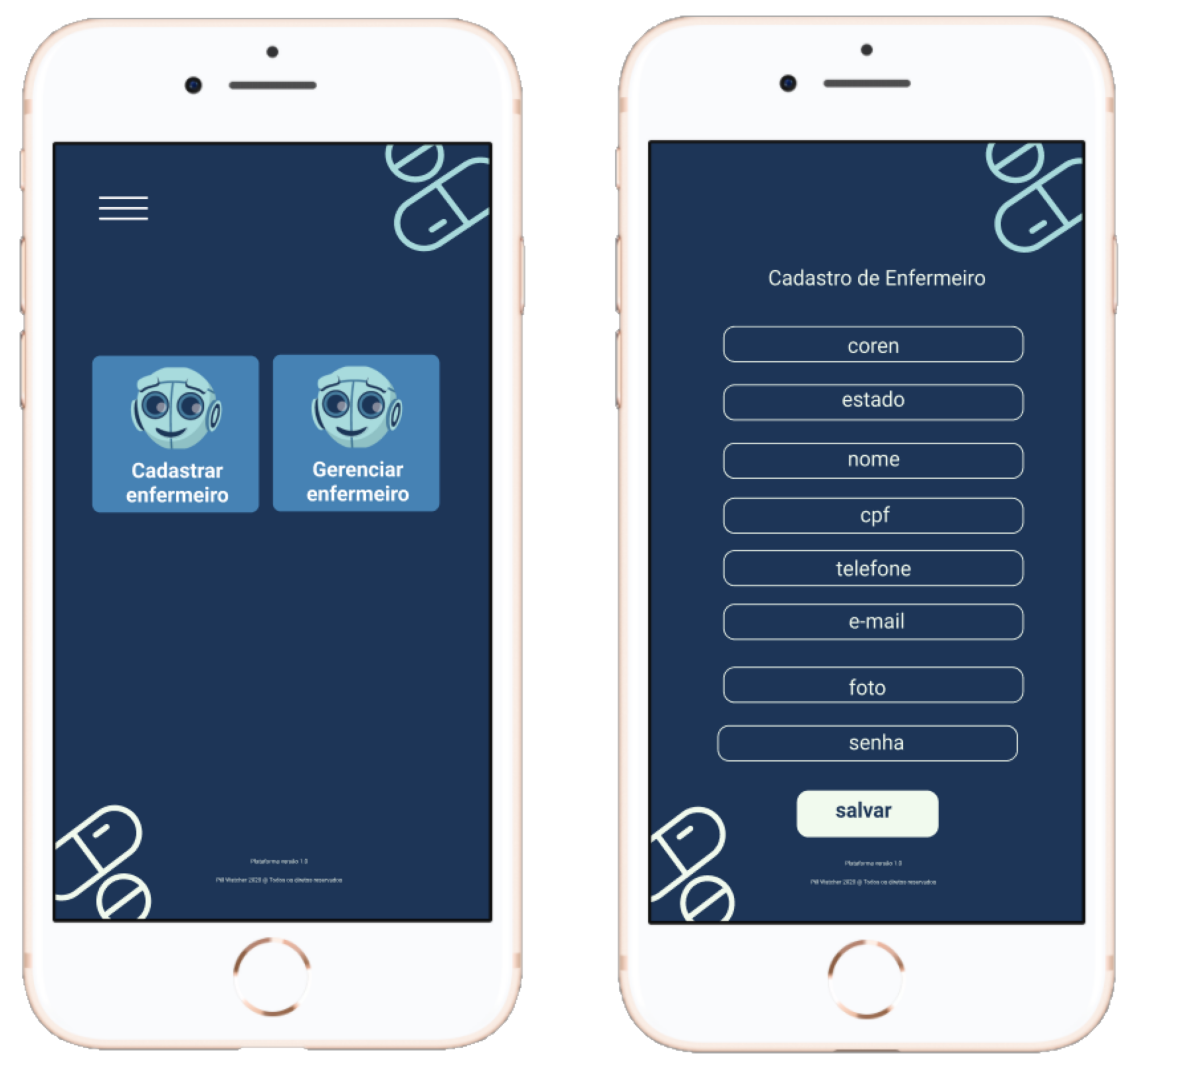
\includegraphics[width=8cm]{figuras/Software_Prototipo/Prototipo_Fluxo_Administrador_2.png}
    \label{fig:prototipo_menu_admin_e_tela_1_cadastro_enfermeiro}}
    \caption{Administrador - Parte 1}
\end{figure}

A figura \ref{fig:prototipo_sidebar_e_alterar_dados} representa a \textit{sidebar} do administrador que contém a foto de perfil, o tipo de usuário, o CPF, o telefone e as opções de editar perfil e sair. Caso o usuário selecione editar perfil, será apresentada a segunda tela onde o usuário pode alterar os dados que foram cadastrados. Já a figura \ref{fig:prototipo_menu_admin_e_tela_1_cadastro_enfermeiro} apresenta o menu inicial do administrador, onde o possibilita de cadastrar um(a) enfermeiro(a) e gerenciar os enfermeiros cadastrados. Por fim, a última tela demonstra a primeira etapa do cadastro de um enfermeiro.

\begin{figure}[H]
    \centering
    \subfloat[][Etapa 2 do cadastro de enfermeiro(a) e \\ tela 1 do gerenciamento de enfermeiros]{
    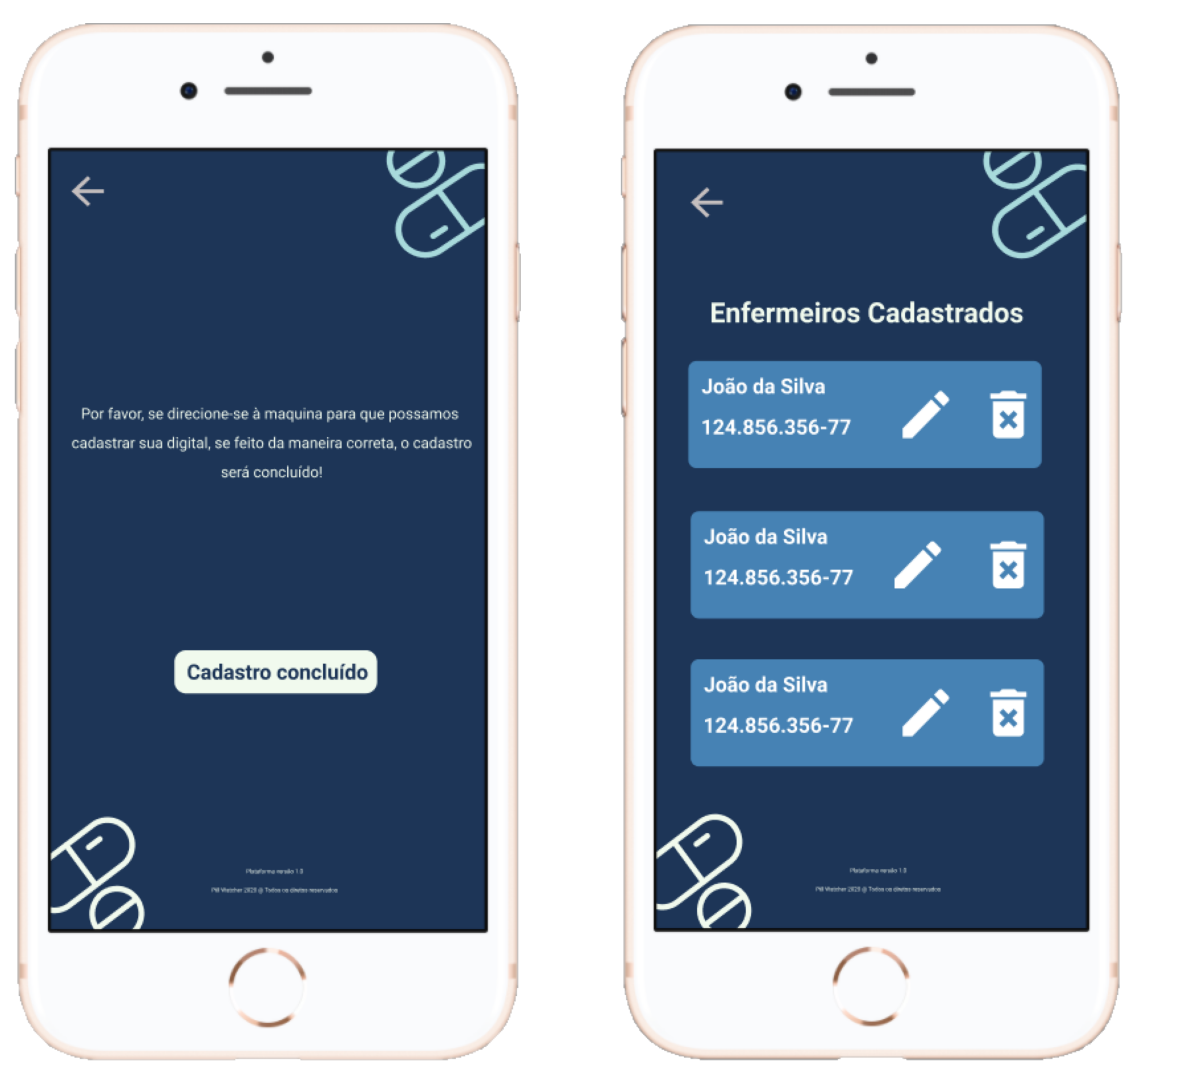
\includegraphics[width=8cm]{figuras/Software_Prototipo/Prototipo_Fluxo_Administrador_3.png}
    \label{fig:prototipo_tela_2_cadastro_enfermeiro_e_tela_1_gerenciamento_enfermeiros}}
\end{figure}

 \begin{figure}[H]
    \centering   
    \subfloat[][Alterar dados do(a) enfermeiro(a) e tela 1 do fluxo \\ de deletar um(a) enfermeiro(a)]{
    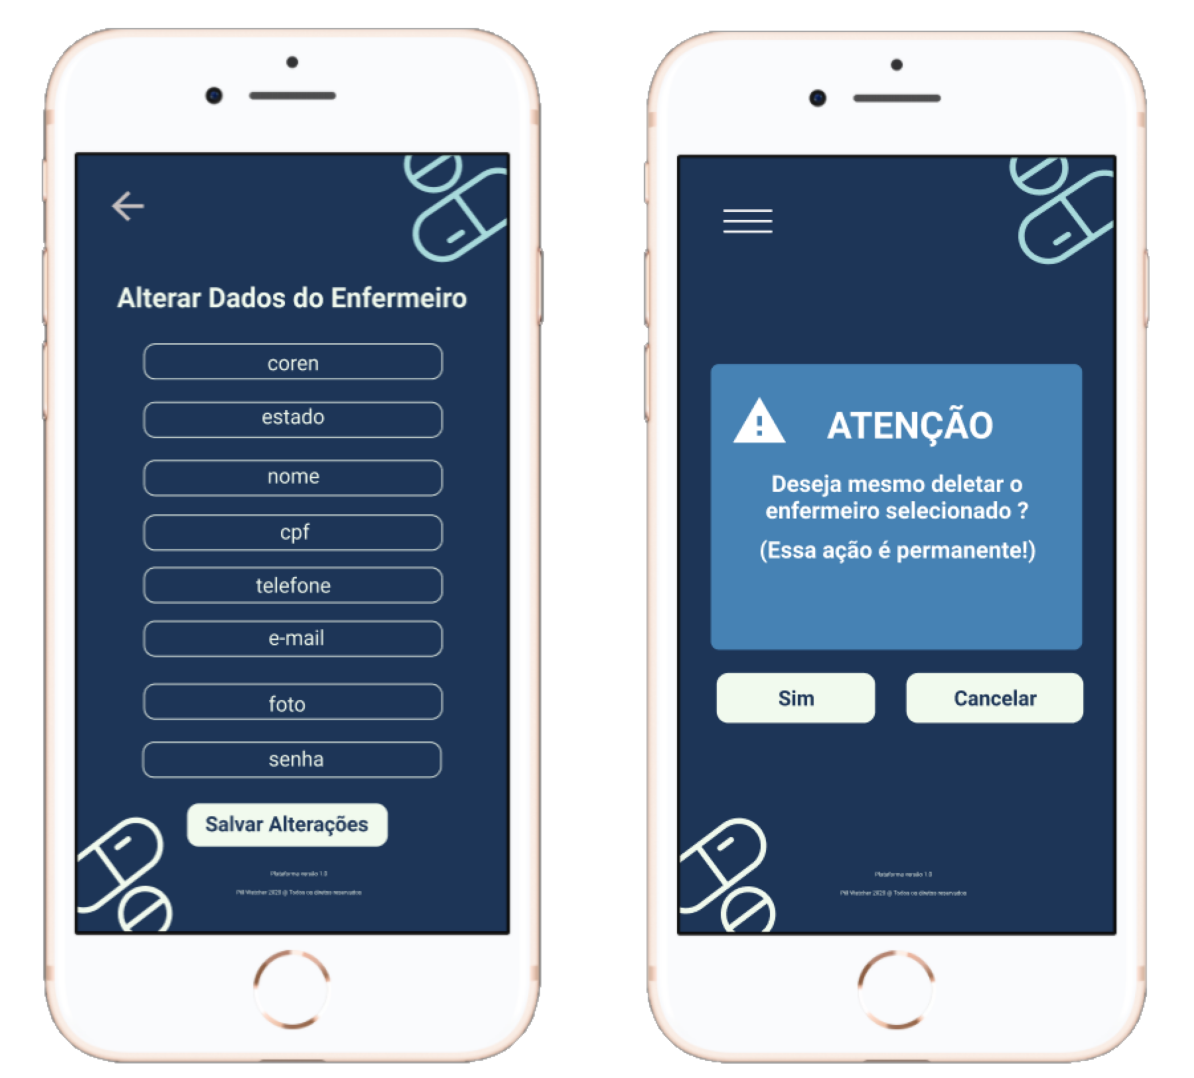
\includegraphics[width=8cm]{figuras/Software_Prototipo/Prototipo_Fluxo_Administrador_4.png}
    \label{fig:prototipo_alterar_dados_enfermeiro_e_tela_1_deletar_enfermeiro}}
     \caption{Administrador - Parte 2}
\end{figure}

Na imagem \ref{fig:prototipo_tela_2_cadastro_enfermeiro_e_tela_1_gerenciamento_enfermeiros} são retratadas a etapa 2 de cadastro de enfermeiro que solicita que o usuário se dirija até a máquina para registrar sua identidade biométrica e a primeira tela do fluxo de gerenciamento de enfermeiros que lista todos os enfermeiros cadastrados e para cada um é possível editar os dados ou deletá-lo do sistema. A gravura \ref{fig:prototipo_alterar_dados_enfermeiro_e_tela_1_deletar_enfermeiro} demonstra, caso essa alternativa tenha sido selecionada na tela anterior, a tela de editar os dados e a primeira tela do fluxo de deletar um enfermeiro do sistema que solicita a confirmação do usuário para completar essa ação.

 A Tela \ref{fig:prototipo_tela_2_deletar_enfermeiro} é responsável por fornecer o \textit{feedback} de completude da ação de apagar um enfermeiro do sistema.
 
\begin{figure}[H]
    \centering
    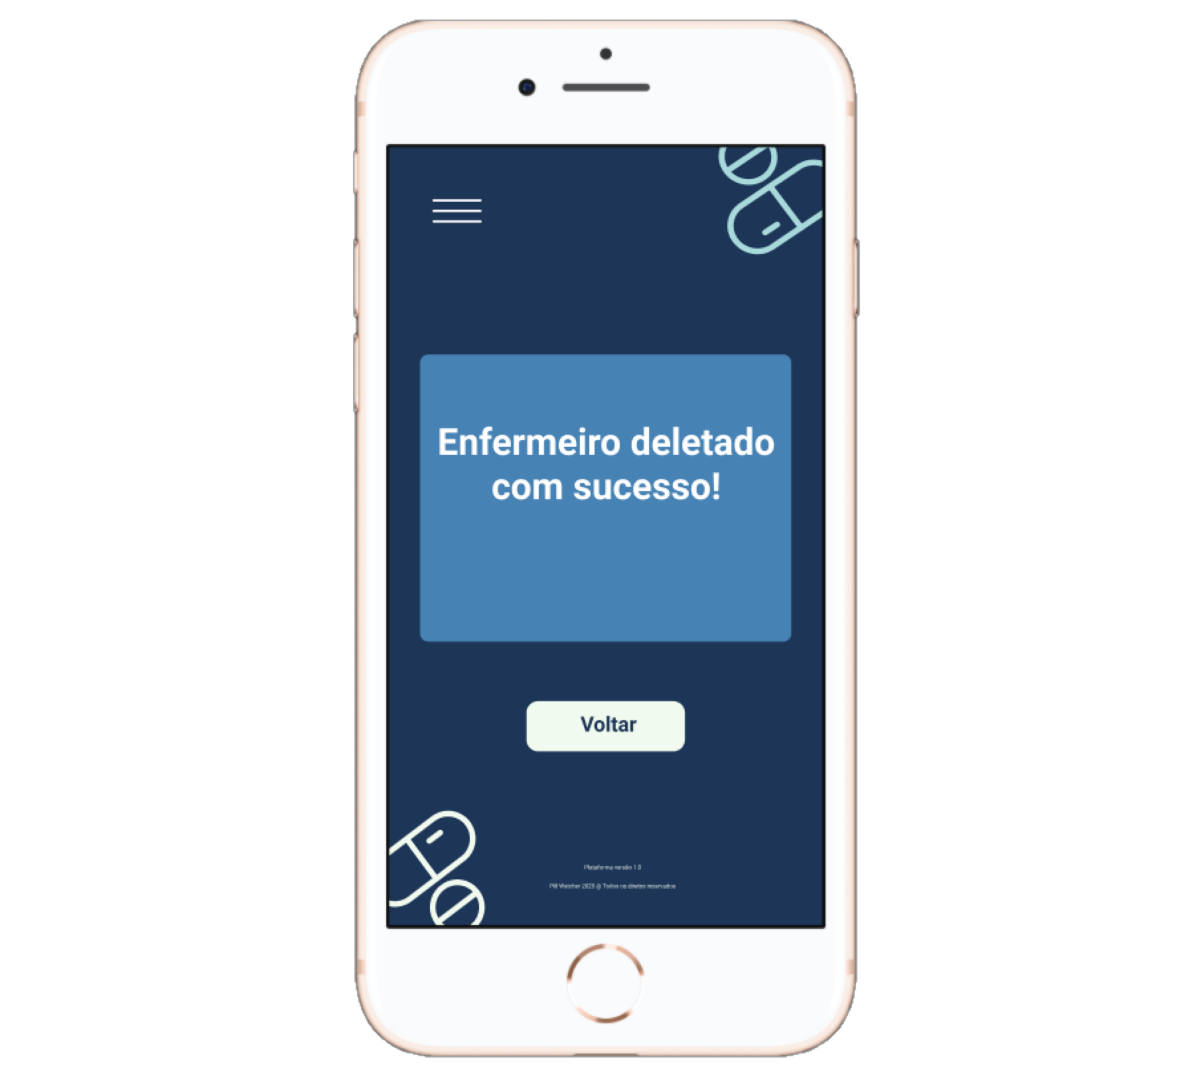
\includegraphics[width=8cm]{figuras/Software_Prototipo/Prototipo_Fluxo_Administrador_5.png}
    \caption{Administrador - Parte 3}
    \label{fig:prototipo_tela_2_deletar_enfermeiro}
\end{figure}


\subsection{Enfermeiro(a)}
\begin{figure}[H]
    \centering
    \subfloat[][Sidebar e tela para alterar dados do perfil]{
    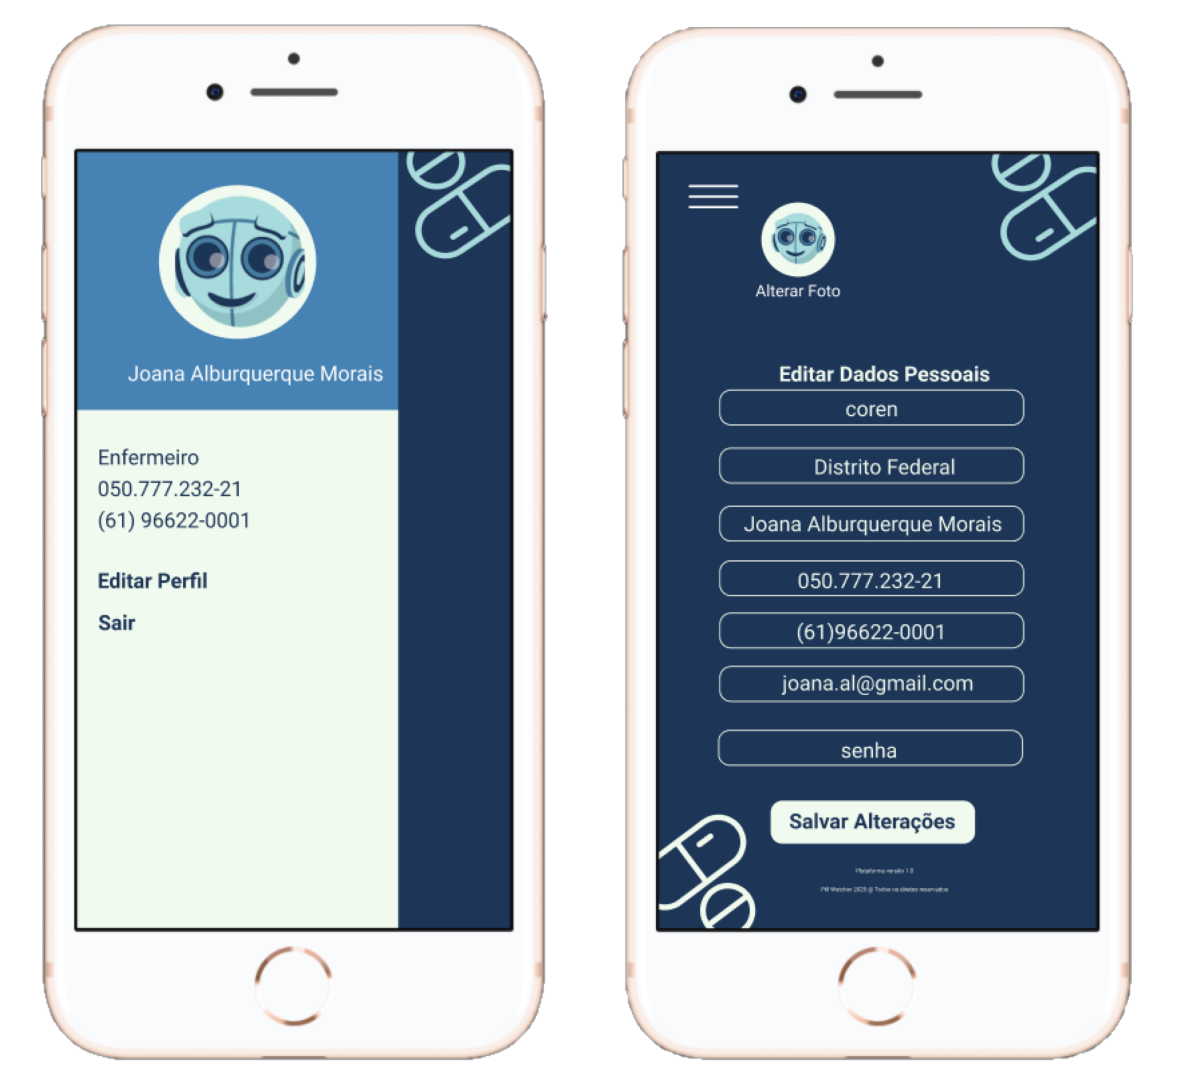
\includegraphics[width=8cm]{figuras/Software_Prototipo/Prototipo_Fluxo_Enfermeiro_1.png}
    \label{fig:prototipo_enfermeiro_sidebar_e_alterar_perfil}}
\end{figure}

\begin{figure}[H]
    \centering
    \subfloat[][Menu inicial e tela 1 de gerenciar pacientes]{
    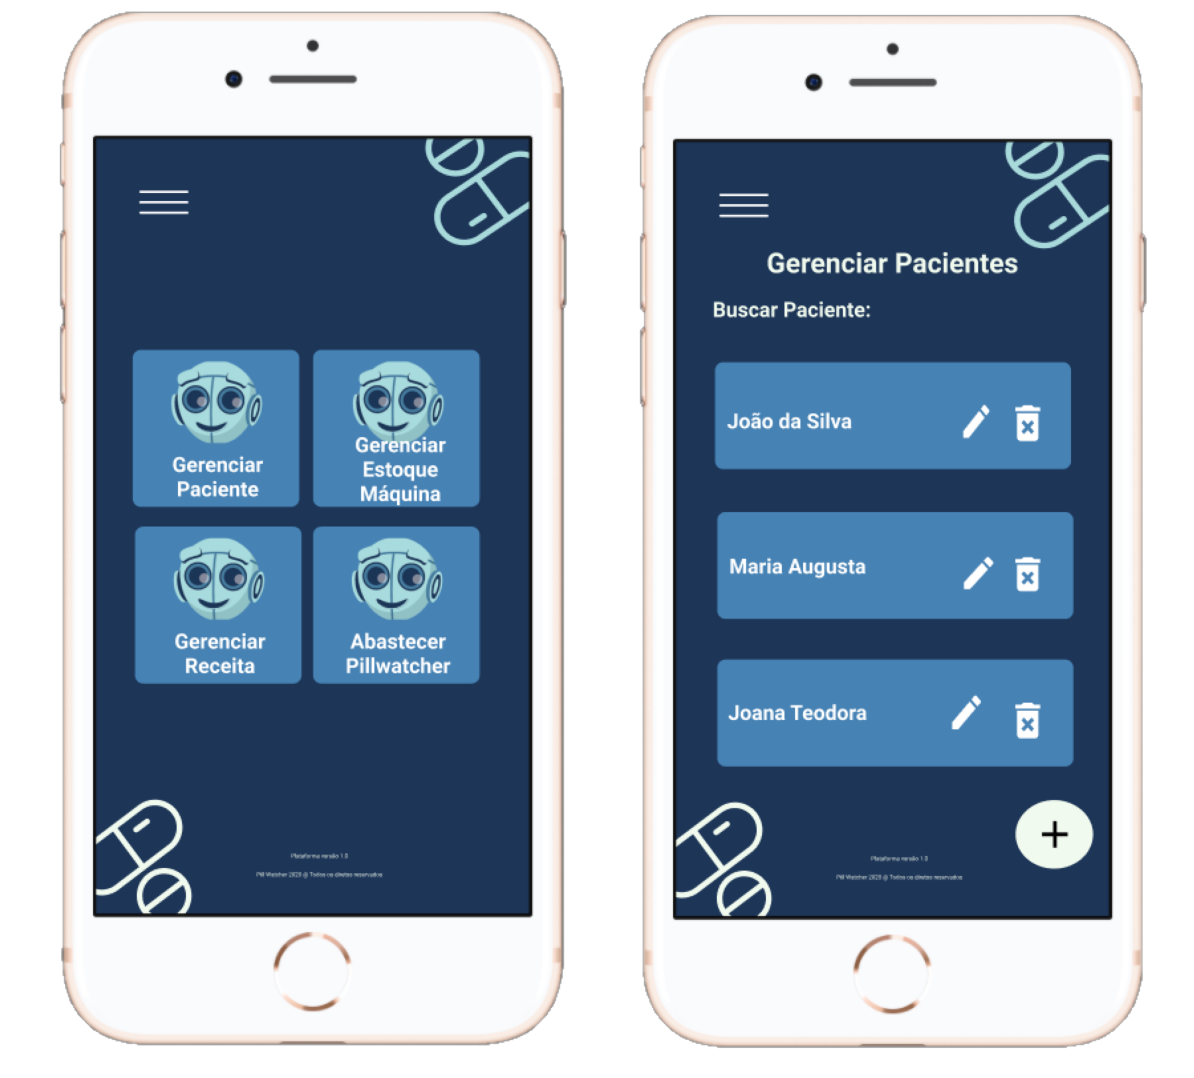
\includegraphics[width=8cm]{figuras/Software_Prototipo/Prototipo_Fluxo_Enfermeiro_2.png}
    \label{fig:prototipo_enfermeiro_menu_e_tela_1_gerenciar_pacientes}}
    \caption{Enfermeiro - Parte 1}
\end{figure}

Após a realização do login por parte do enfermeiro, o próprio será direcionado para o menu inicial, onde terá as opções de gerenciamento. No canto superior esquerdo, encontra-se o link para a \textit{sidebar}, a qual terá a opção de sair e de editar dados do usuário. No menu principal, encontra-se a opção de gerenciar paciente, uma das mais importantes, que é representado pela tela \ref{fig:prototipo_enfermeiro_menu_e_tela_1_gerenciar_pacientes}. Nessa tela, as funcionalidades servem para dar ao enfermeiro total controle dos dados do paciente. 

\begin{figure}[H]
    \centering
    \subfloat[][Etapa 1 e 2 de cadastro de um paciente]{
    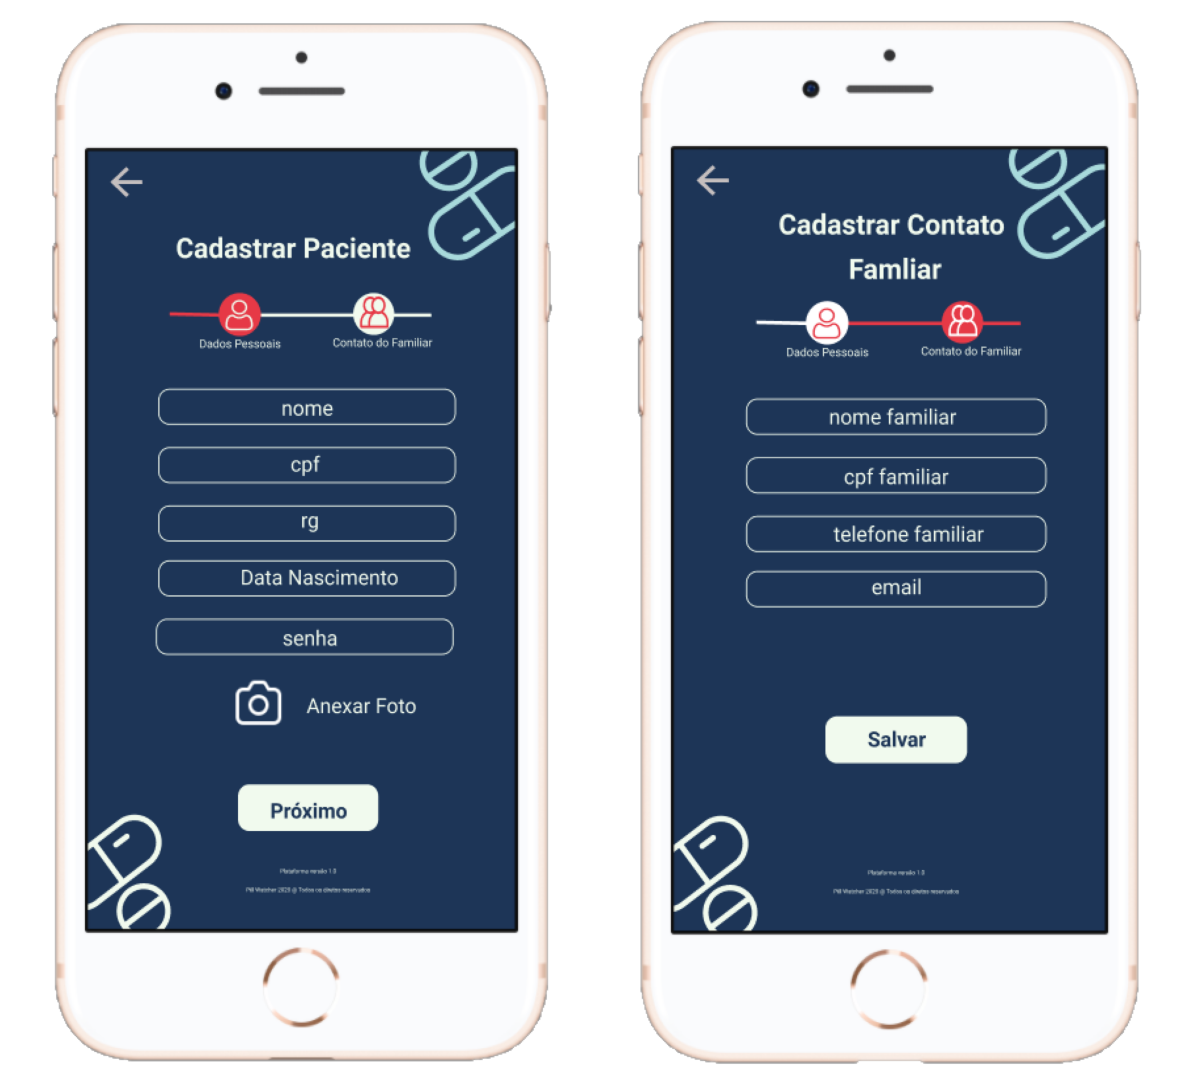
\includegraphics[width=8cm]{figuras/Software_Prototipo/Prototipo_Fluxo_Enfermeiro_3.png}
    \label{fig:prototipo_enfermeiro_cadastro_paciente}}
\end{figure}

\begin{figure}[H]
    \centering   
    \subfloat[][Etapa 1 e 2 para alterar dados de um paciente]{
    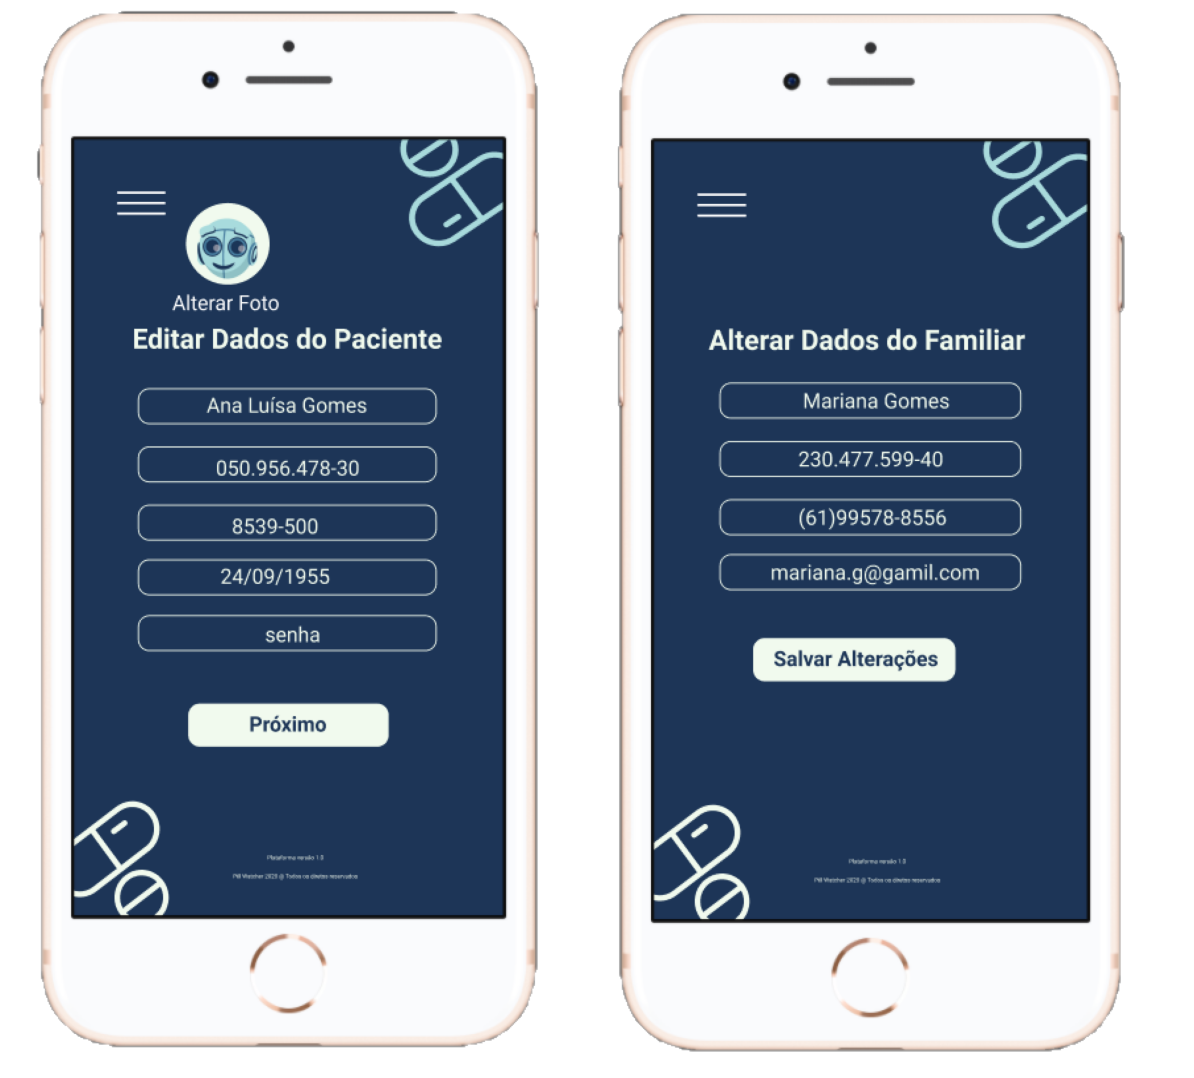
\includegraphics[width=8cm]{figuras/Software_Prototipo/Prototipo_Fluxo_Enfermeiro_4.png}
    \label{fig:prototipo_enfermeiro_alterar_dados}}
    \caption{Enfermeiro - Parte 2}
\end{figure}


As telas referentes à imagem \ref{fig:prototipo_enfermeiro_cadastro_paciente} referem-se ao cadastro de paciente, que fora divido em duas partes. A primeira diz respeito onde os dados do paciente são colocados e a segunda onde se inserem os dados de algum familiar responsável.

Na terceira tela da imagem \ref{fig:prototipo_enfermeiro_alterar_dados} o enfermeiro pode editar os dados de paciente. O paciente não terá essa opção. O próprio deverá entrar em contato com o enfermeiro e informar os dados que serão atualizados. A quarta tela da imagem \ref{fig:prototipo_enfermeiro_alterar_dados} é para a edição dos dados do familiar, que será feito da mesma forma dos dados do paciente.

A primeira e segunda tela da imagem \ref{fig:prototipo_enfermeiro_deletar_paciente} mostram um fluxo de deleção de algum paciente. Quando um enfermeiro clicar em excluir, uma mensagem de atenção aparecerá, e, se o enfermeiro clicar na opção 'Sim', a tela \ref{fig:prototipo_enfermeiro_deletar_paciente} de confirmação de deleção será mostrada, com a opção de voltar para a tela de gerenciamento de paciente.

O enfermeiro possui também a opção de gerenciar o estoque da máquina, através do menu inicial clicando em um botão chamado "Gerenciar Estoque". Tal botão conecta-se com a tela \ref{fig:prototipo_enfermeiro_tela_inicial_gerenciar_estoque_medicamento_e_inserir_novo_medicamento}. O gerenciamento de estoque possui o mesmo padrão de gerenciamento de paciente, onde é possível inserir um novo medicamento. Para tal, a tela \ref{fig:prototipo_enfermeiro_tela_inicial_gerenciar_estoque_medicamento_e_inserir_novo_medicamento} foi elaborada para isso.

\begin{figure}[H]
    \centering
    \subfloat[][Fluxo para deletar um paciente do App]{
    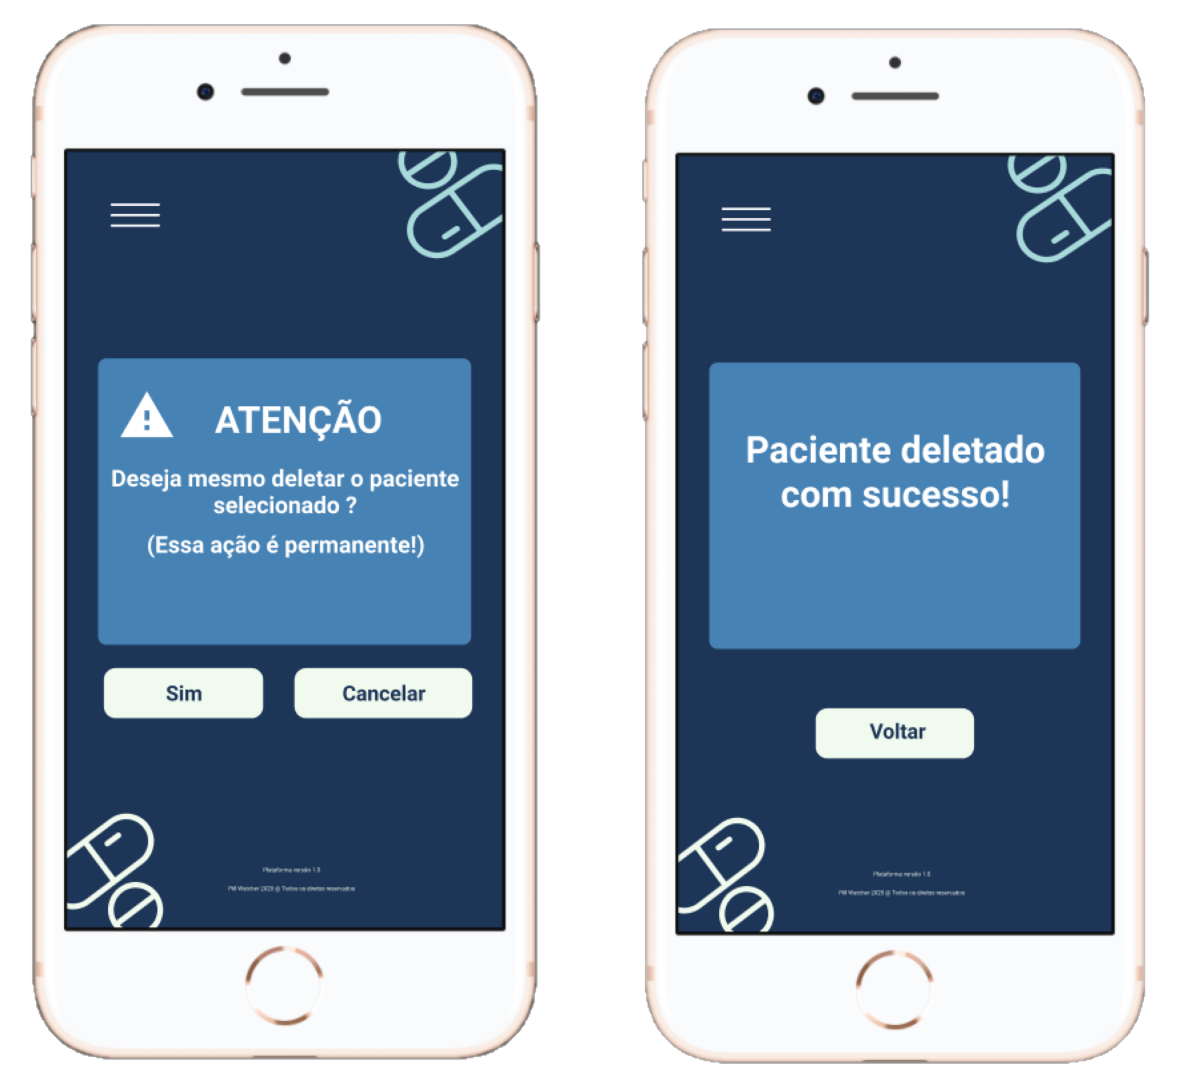
\includegraphics[width=8cm]{figuras/Software_Prototipo/Prototipo_Fluxo_Enfermeiro_5.png}
    \label{fig:prototipo_enfermeiro_deletar_paciente}}
\end{figure}

\begin{figure}[H]
    \centering    
    \subfloat[][Tela inicial de gerenciar estoque da máquina e tela para inserir novo medicamento na máquina]{
    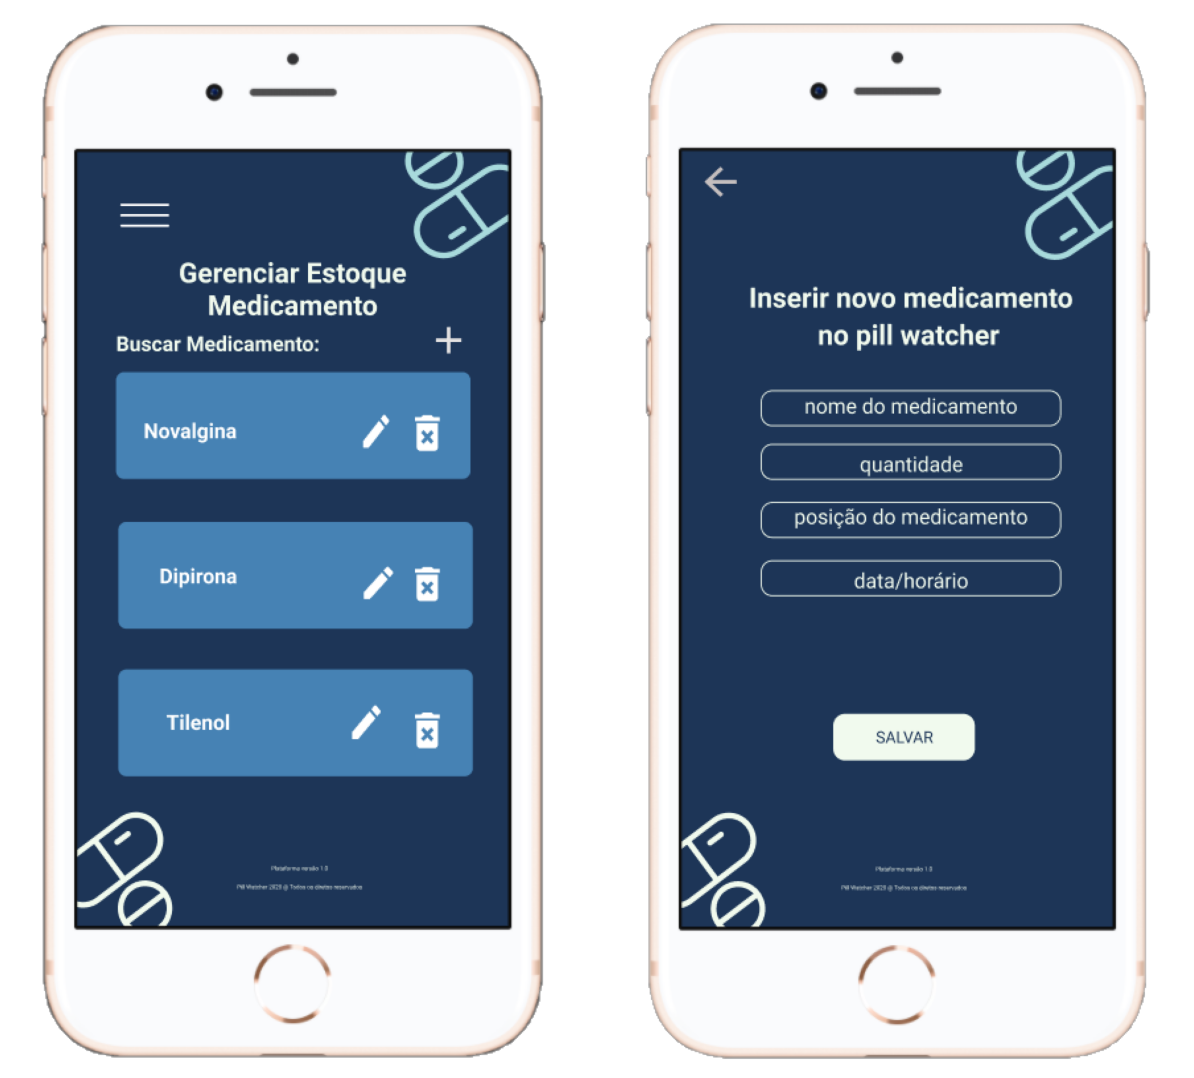
\includegraphics[width=8cm]{figuras/Software_Prototipo/Prototipo_Fluxo_Enfermeiro_6.png}
    \label{fig:prototipo_enfermeiro_tela_inicial_gerenciar_estoque_medicamento_e_inserir_novo_medicamento}}
    \caption{Enfermeiro - Parte 3}
\end{figure}

\begin{figure}[H]
    \centering
    \subfloat[][Tela para editar dados do medicamento da máquina e tela 1 do fluxo para deletar um medicamento da máquina]{
    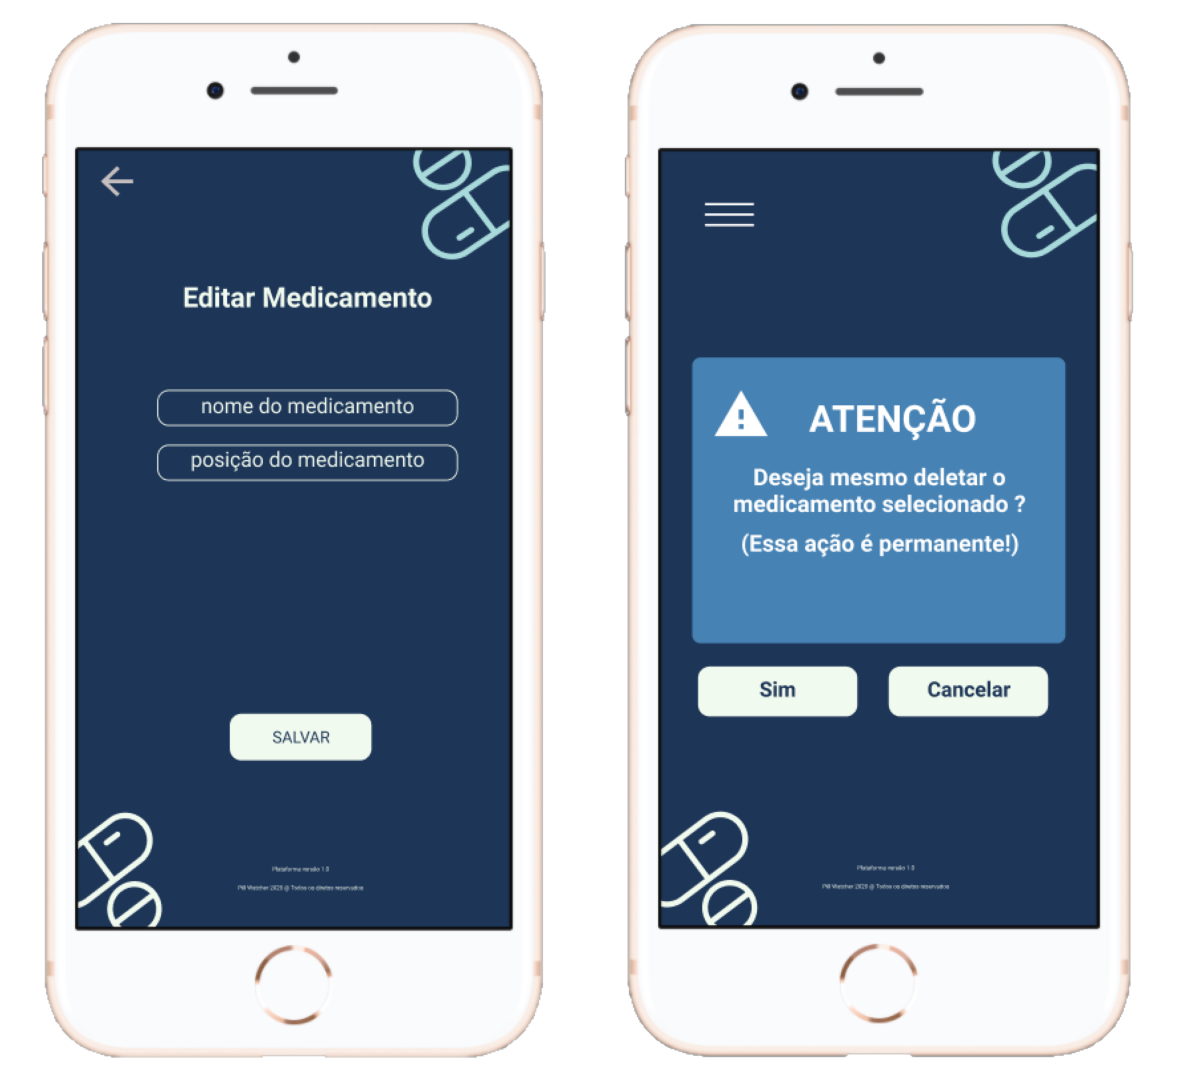
\includegraphics[width=8cm]{figuras/Software_Prototipo/Prototipo_Fluxo_Enfermeiro_7.png}
    \label{fig:prototipo_enfermeiro_editar_dados_medicamento_e_tela_1_do_fluxo_deletar_medicamento}}
\end{figure} 

\begin{figure}[H]
    \centering
    \subfloat[][Tela 2 do fluxo para deletar um medicamento da máquina e tela 1 do fluxo de Gerenciar Receita]{
    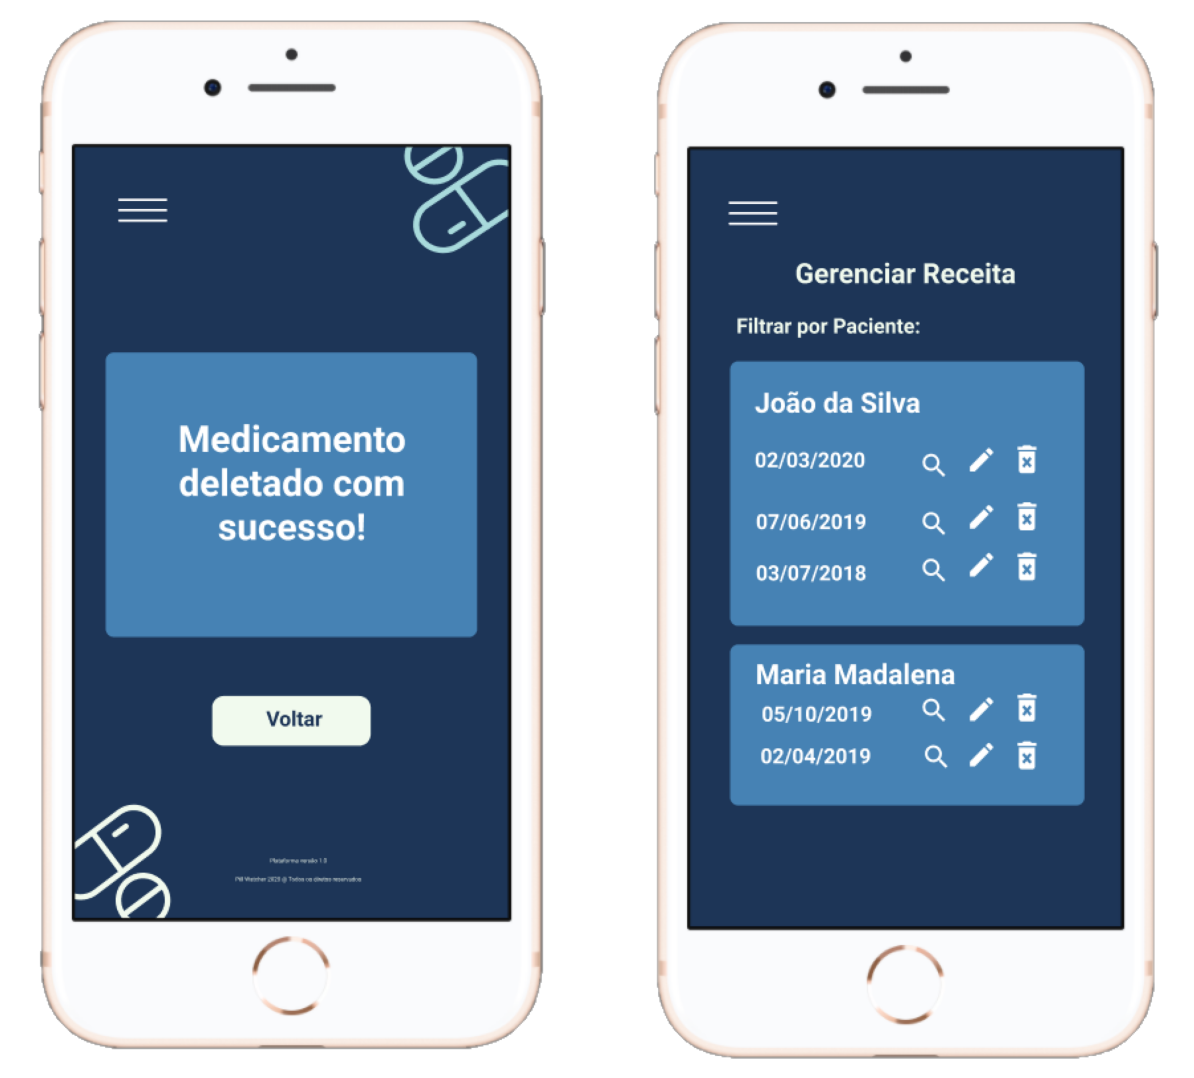
\includegraphics[width=8cm]{figuras/Software_Prototipo/Prototipo_Fluxo_Enfermeiro_8.png}
    \label{fig:prototipo_enfermeiro_tela_2_do_fluxo_deletar_medicamento_e_tela_1_fluxo_gerenciar_receita}}
    \caption{Enfermeiro - Parte 4}
\end{figure}

A primeira tela da imagem \ref{fig:prototipo_enfermeiro_editar_dados_medicamento_e_tela_1_do_fluxo_deletar_medicamento} contém os campos onde o enfermeiro poderá atualizar os dados de medicamento na máquina. A segunda tela apresenta a ação de deletar um medicamento, o qual, por sua vez, verifica se o medicamento realmente deve ser deletado. Caso o enfermeiro clique na opção 'Sim', a tela de confirmação aparecerá, com o botão voltar, que permite ao usuário voltar para a página de gerenciamento de medicamentos.

A imagem \ref{fig:prototipo_enfermeiro_tela_2_do_fluxo_deletar_medicamento_e_tela_1_fluxo_gerenciar_receita} mostra a funcionalidade de gerenciar receita de paciente, com o nome do paciente seguido dos remédios que o próprio toma. Os botões de deletar, editar e adicionar receita estão presentes nessa página.

\begin{figure}[H]
    \centering
    \subfloat[][Visualizar receita e tela 1 do fluxo para cadastrar uma receita]{
    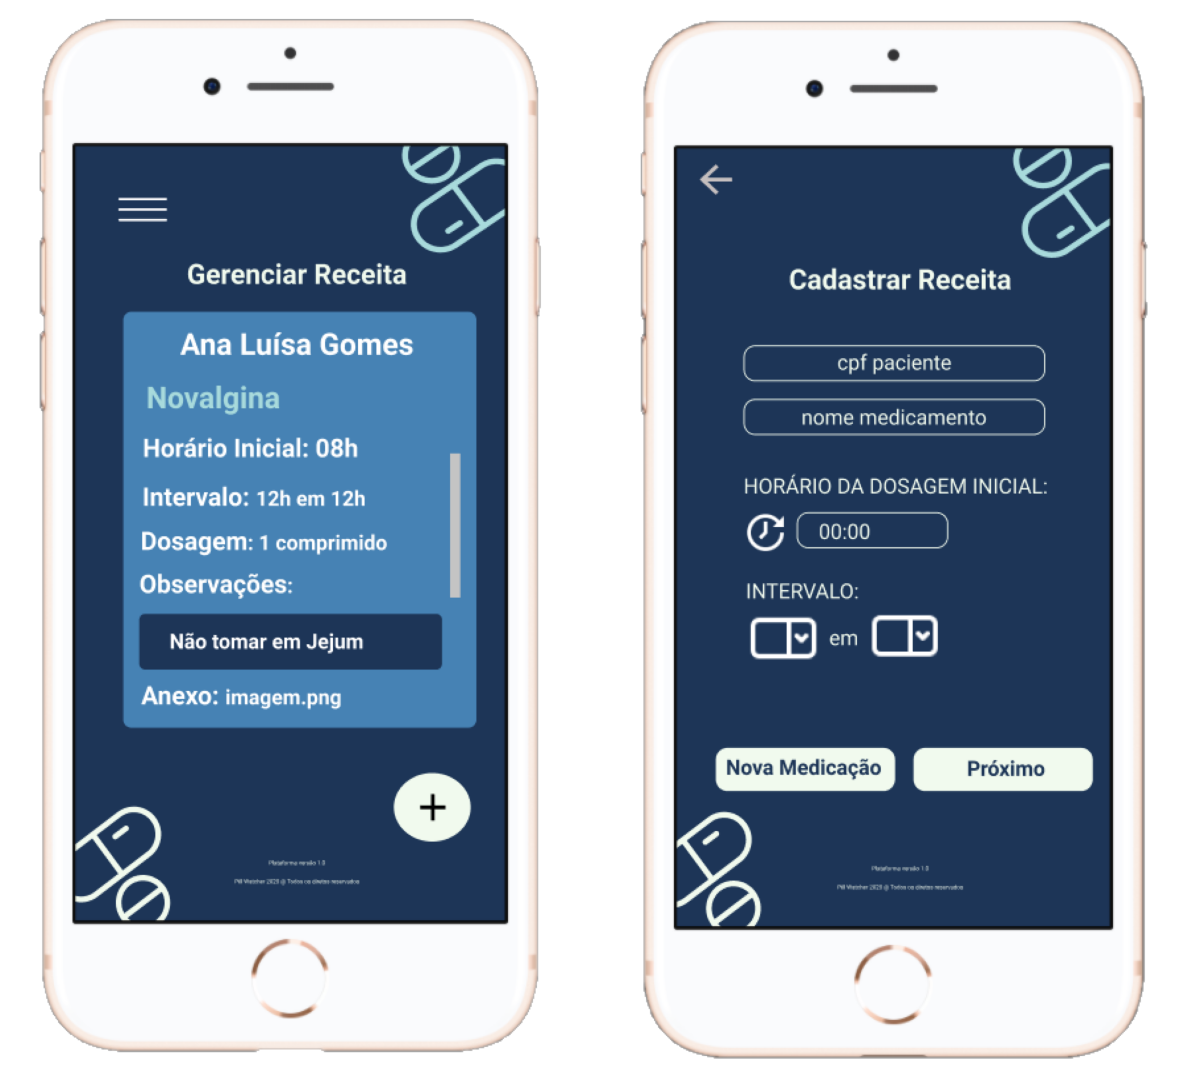
\includegraphics[width=8cm]{figuras/Software_Prototipo/Prototipo_Fluxo_Enfermeiro_9.png}
    \label{fig:prototipo_enfermeiro_visualizar_receita_e_tela_1_fluxo_cadastrar_receita}}
\end{figure}

\begin{figure}[H]
    \centering
    \subfloat[][Tela 2 e 3 do fluxo para cadastrar uma receita ]{
    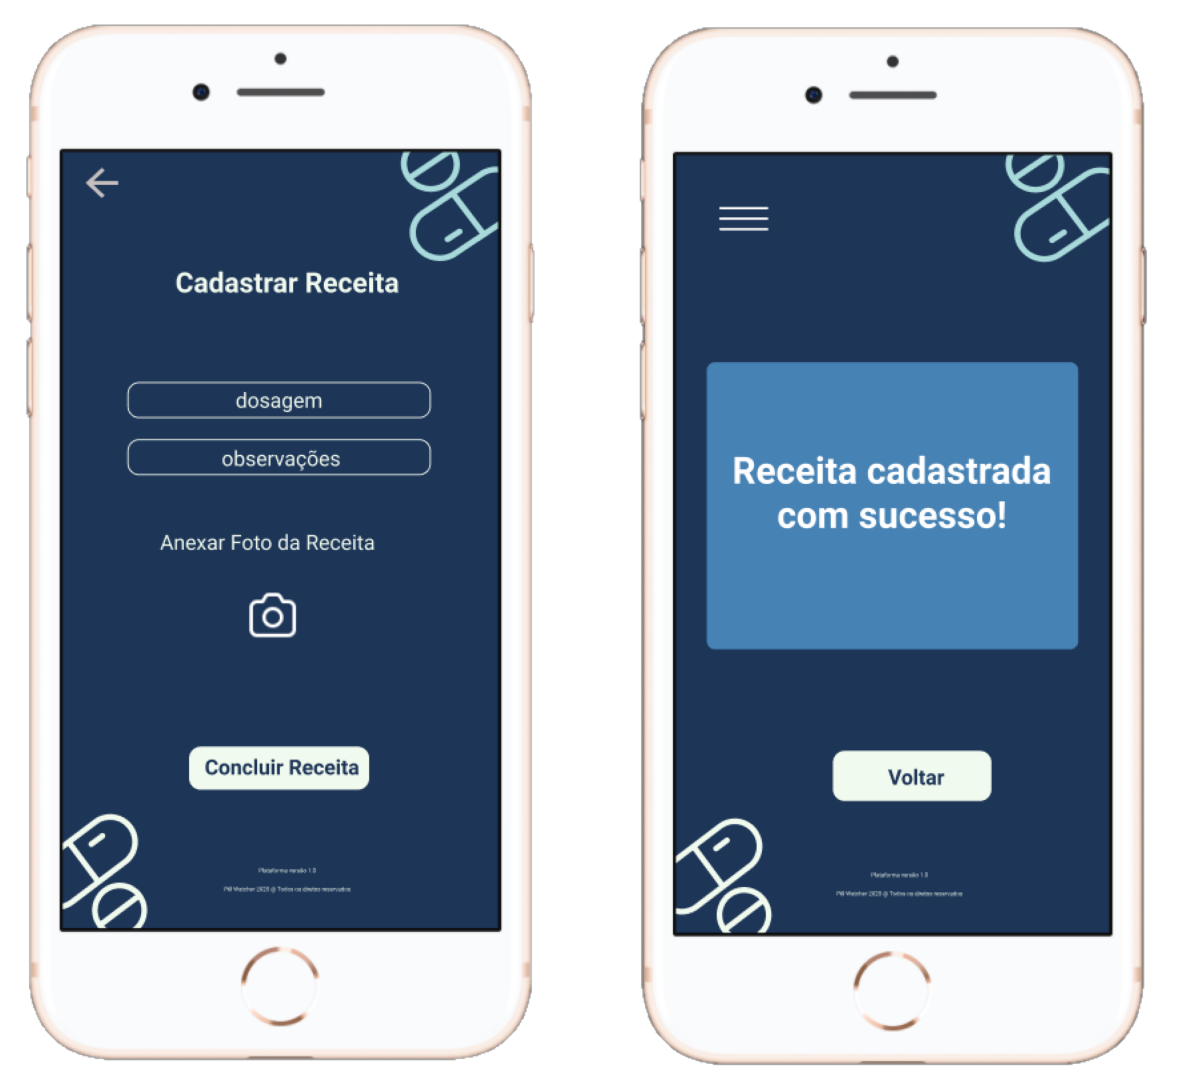
\includegraphics[width=8cm]{figuras/Software_Prototipo/Prototipo_Fluxo_Enfermeiro_10.png}
    \label{fig:prototipo_enfermeiro_tela_2_e_3_do_fluxo_cadastrar_receita}}
    \caption{Enfermeiro - Parte 5}
\end{figure}

Ao clicar em uma receita específica, a primeira tela da imagem \ref{fig:prototipo_enfermeiro_visualizar_receita_e_tela_1_fluxo_cadastrar_receita} aparecerá, com as informações de cada medicamento. A segunda tela mostra o cadastro de receita, que é feito em duas etapas. A segunda, terceira e quarta tela mostram o fluxo completo. Por fim, a quarta tela diz respeito à confirmação do cadastro.

Quando o enfermeiro clicar no botão de editar dados de receita, a primeira tela da imagem \ref{fig:prototipo_enfermeiro_alterar_dados_receita_e_tela_1_fluxo_deletar_receita} aparecerá. Após a inicialização da tela, é realizada a atualização dos dados. A segunda e terceira tela representam o fluxo de deleção de receita, onde a primeira diz respeito à confirmação por parte do usuário e a segunda evidencia que a receita fora realmente deletada.

\begin{figure}[H]
    \centering
    \subfloat[][Tela para alterar dados da receita e tela 1 do \\ fluxo para deletar uma receita]{
    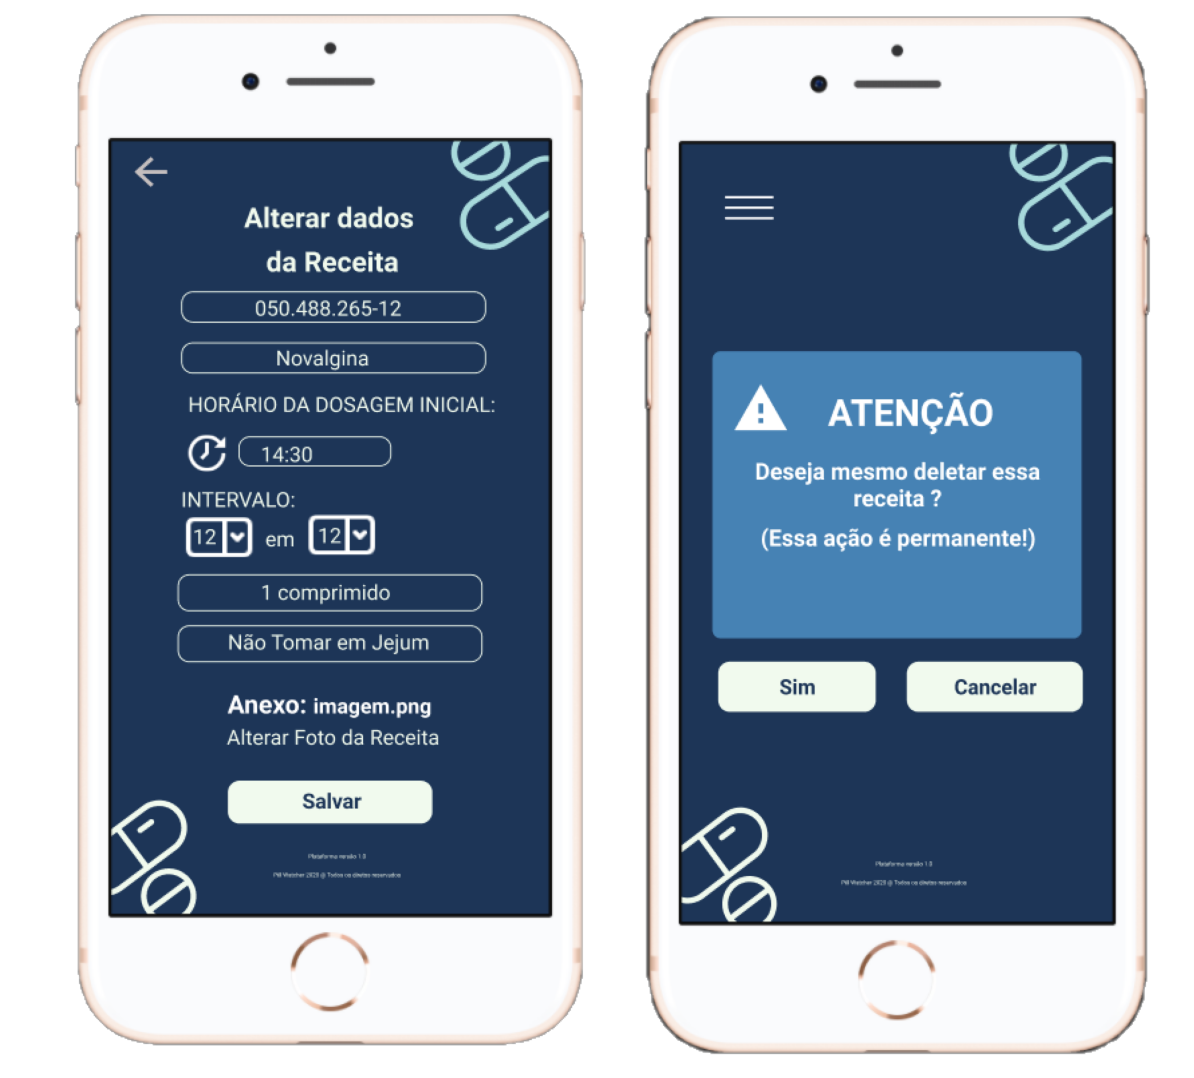
\includegraphics[width=8cm]{figuras/Software_Prototipo/Prototipo_Fluxo_Enfermeiro_11.png}
    \label{fig:prototipo_enfermeiro_alterar_dados_receita_e_tela_1_fluxo_deletar_receita}}
\end{figure}
    
\begin{figure}[H]
    \centering    
    \subfloat[][Tela 2 do fluxo para deletar uma receita e tela 1 do fluxo de abastecimento da máquina]{
    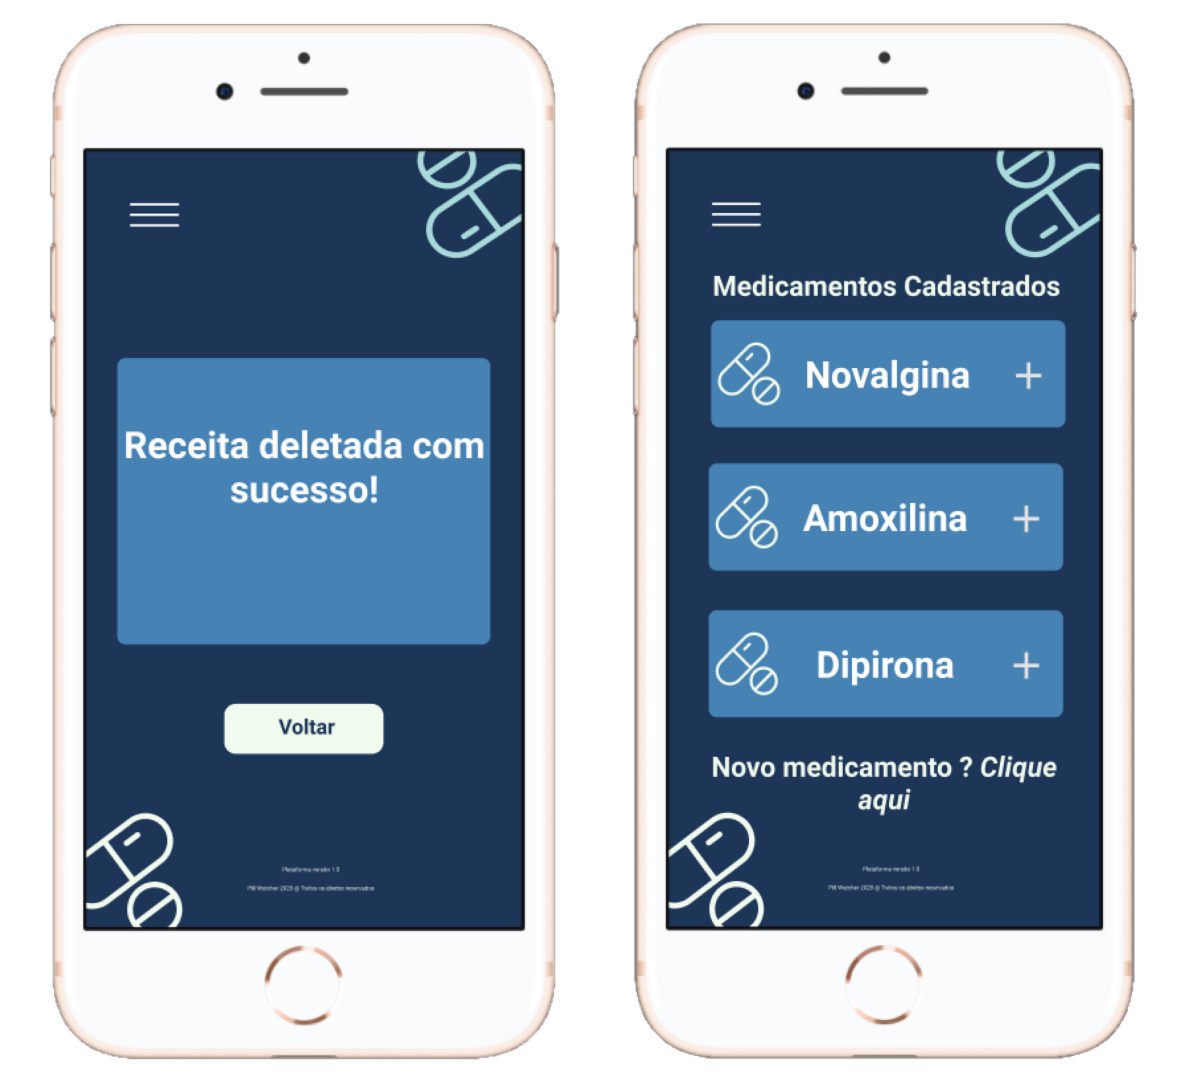
\includegraphics[width=8cm]{figuras/Software_Prototipo/Prototipo_Fluxo_Enfermeiro_12.png}
    \label{fig:prototipo_enfermeiro_tela_2_fluxo_deletar_receita_e_tela_1_fluxo_abastecimento}}
    \caption{Enfermeiro - Parte 6}
\end{figure}



A última tela mostra a lista de medicamentos cadastrados na máquina, onde o enfermeiro pode ser direcionado para a página de adição de medicamento, junto com um botão que chama a tela de cadastro de medicamento.

\begin{figure}[H]
    \centering
    \subfloat[][Telas 2 e 3 do fluxo de abastecimento]{
    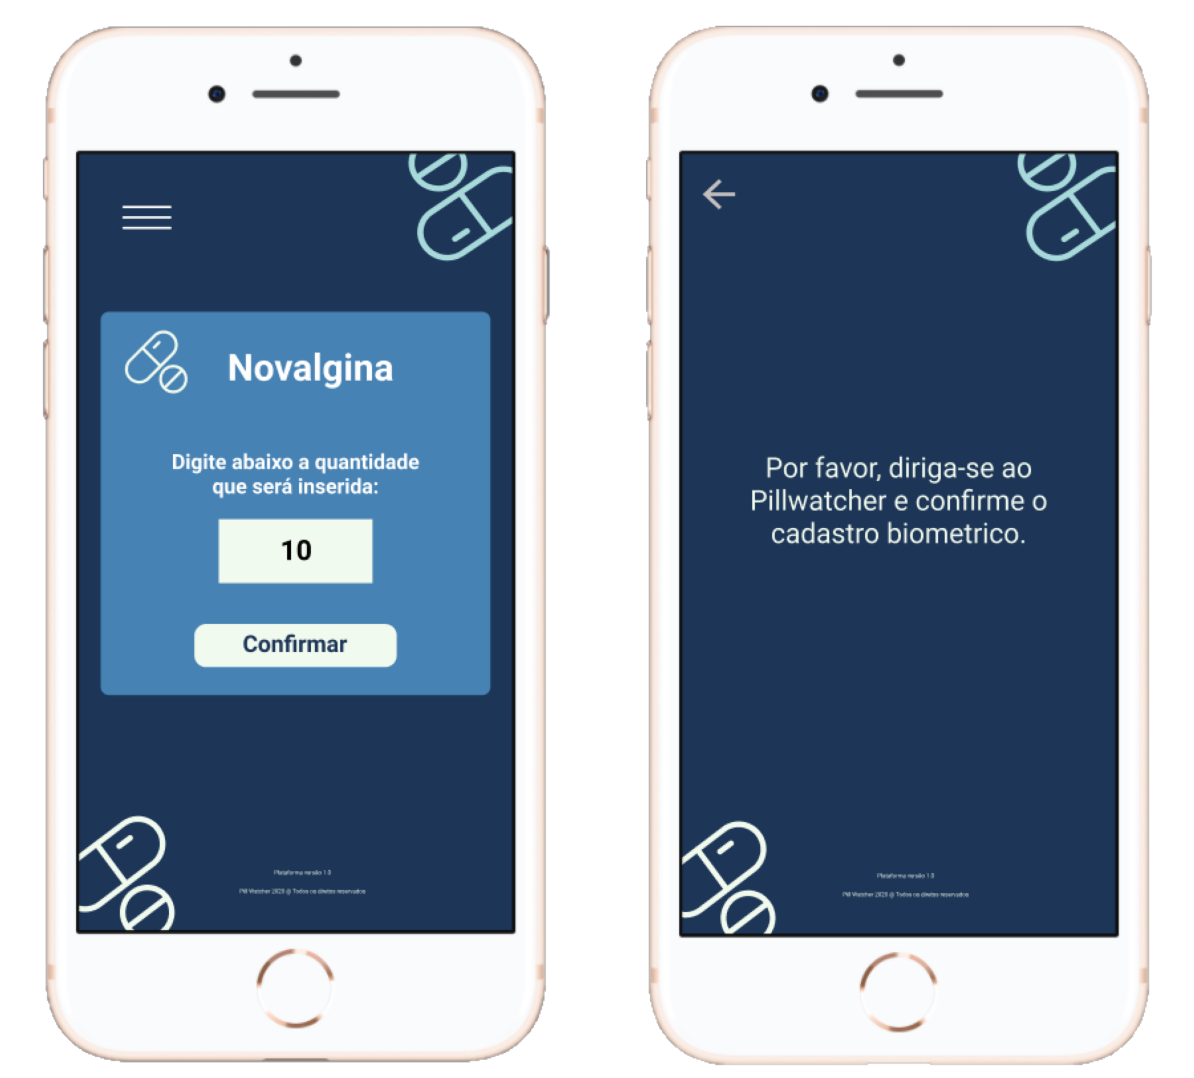
\includegraphics[width=8cm]{figuras/Software_Prototipo/Prototipo_Fluxo_Enfermeiro_13.png}
    \label{fig:prototipo_enfermeiro_telas_2_e_3_fluxo_abastecimento}}
\end{figure}
    
\begin{figure}[H]
    \centering  
    \subfloat[][Telas 4 e 5 do fluxo de abastecimento]{
    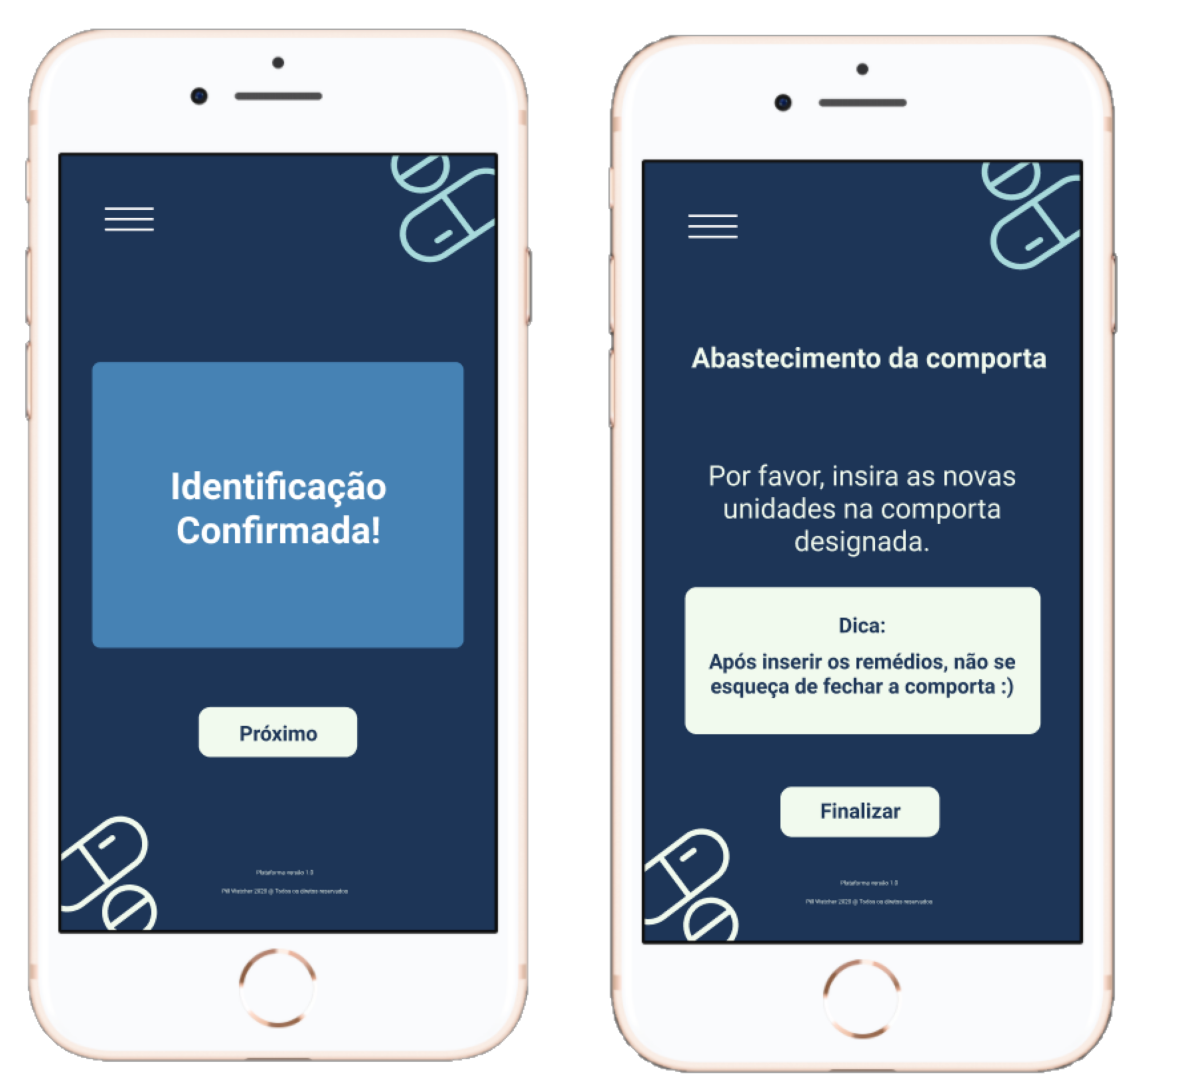
\includegraphics[width=8cm]{figuras/Software_Prototipo/Prototipo_Fluxo_Enfermeiro_14.png}
    \label{fig:prototipo_enfermeiro_telas_4_e_5_fluxo_abastecimento}}
    \caption{Enfermeiro - Parte 7}
\end{figure}

O enfermeiro deve informar a quantidade de cápsulas que serão adicionados na máquina. A segunda tela informa ao usuário que é necessário a confirmação biométrica. Se a confirmação for realizada com sucesso a terceira tela aparecerá, e a quarta tela informará ao usuário que os remédios já poderão ser inseridos na comporta.

\begin{figure}[H]
    \centering
    \subfloat[][Tela 6 do fluxo de abastecimento e tela de notificação de retirada de medicação]{
    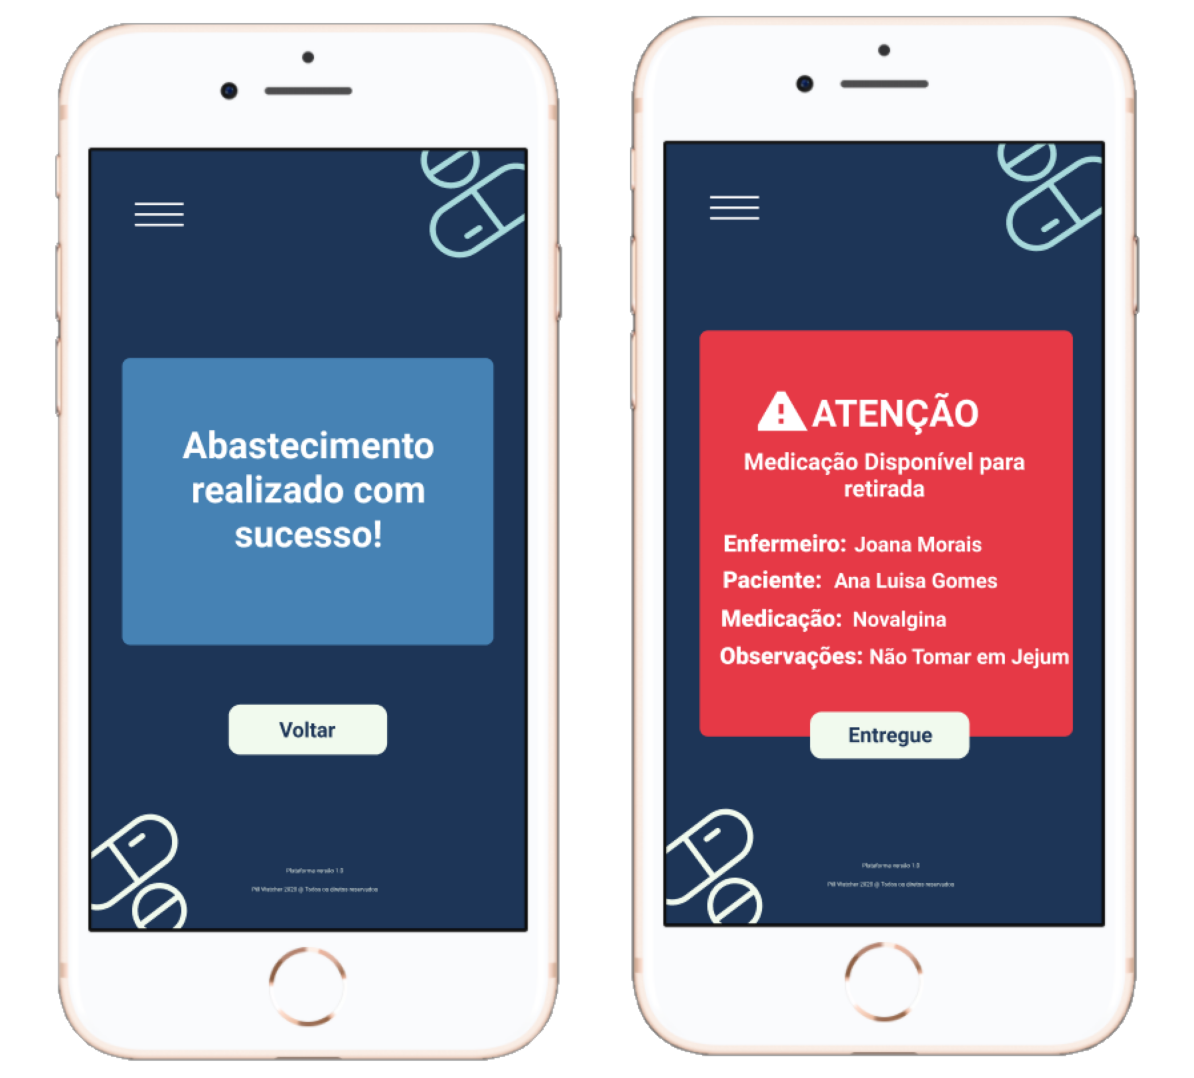
\includegraphics[width=8cm]{figuras/Software_Prototipo/Prototipo_Fluxo_Enfermeiro_15.png}
    \label{fig:prototipo_enfermeiro_tela_6_fluxo_abastecimento_e_retirada_de_medicacao}}
    \caption{Enfermeiro - Parte 8}
\end{figure}

\ref{fig:prototipo_enfermeiro_tela_6_fluxo_abastecimento_e_retirada_de_medicacao} demonstra a tela de \textit{feedback} do abastecimento da máquina e ao lado é apresentado a notificação para retirada de uma medicação na máquina contendo o nome do enfermeiro, o paciente, a medicação e as observações e o botão "Entregue" para o enfermeiro confirmar a entrega da medicação. 

\subsection{Paciente}
Em \ref{fig:prototipo_paciente_sidebar_e_menu_inicial} são representadas a \textit{sidebar} do paciente com a foto, tipo de usuário, CPF, telefone e opções de editar perfil e sair e o menu inicial do paciente que o permite visualizar o estoque e o relatório de medicação. Ao lado (\ref{fig:prototipo_paciente_fluxo_gerencia_estoque_pessoal}), é apresentado o fluxo de visualizar estoque. Na tela 1 é exibido o nome do paciente, todas as suas medicações juntamente com a opção de mostrar mais detalhes sobre essa, caso esse caminho seja acionado, é mostrado o nome do paciente, o nome da medicação, o horário, os dias, a quantidade disponível e o nível do estoque.

\begin{figure}[H]
    \centering
    \subfloat[][Sidebar e menu inicial]{
    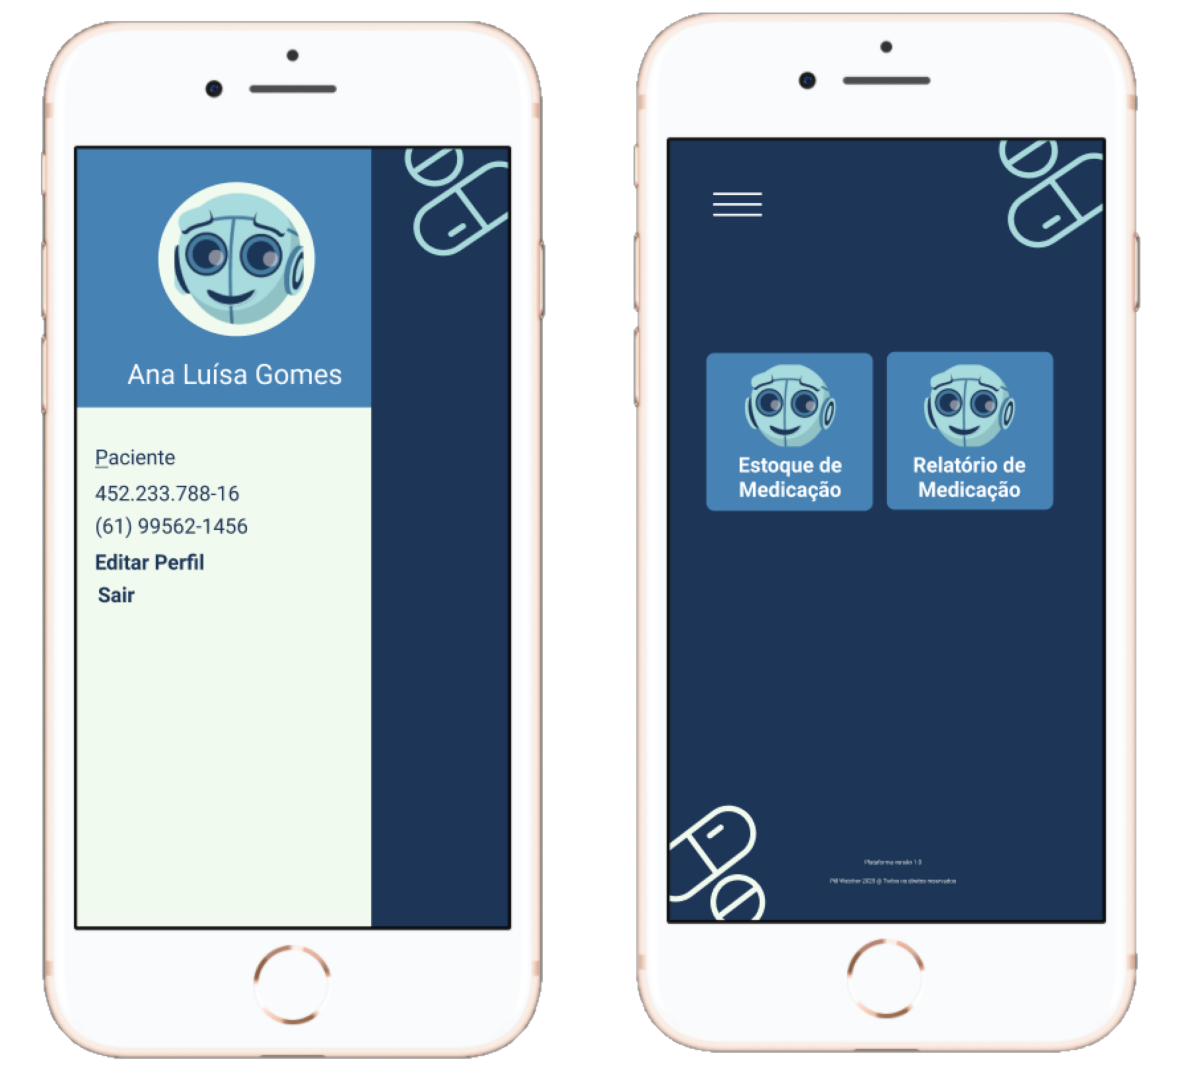
\includegraphics[width=8cm]{figuras/Software_Prototipo/Prototipo_Fluxo_Paciente_1.png}
    \label{fig:prototipo_paciente_sidebar_e_menu_inicial}}
\end{figure}
    
\begin{figure}[H]
    \centering 
    \subfloat[][Tela 1 e 2 do Gerenciamento de Estoque Pessoal]{
    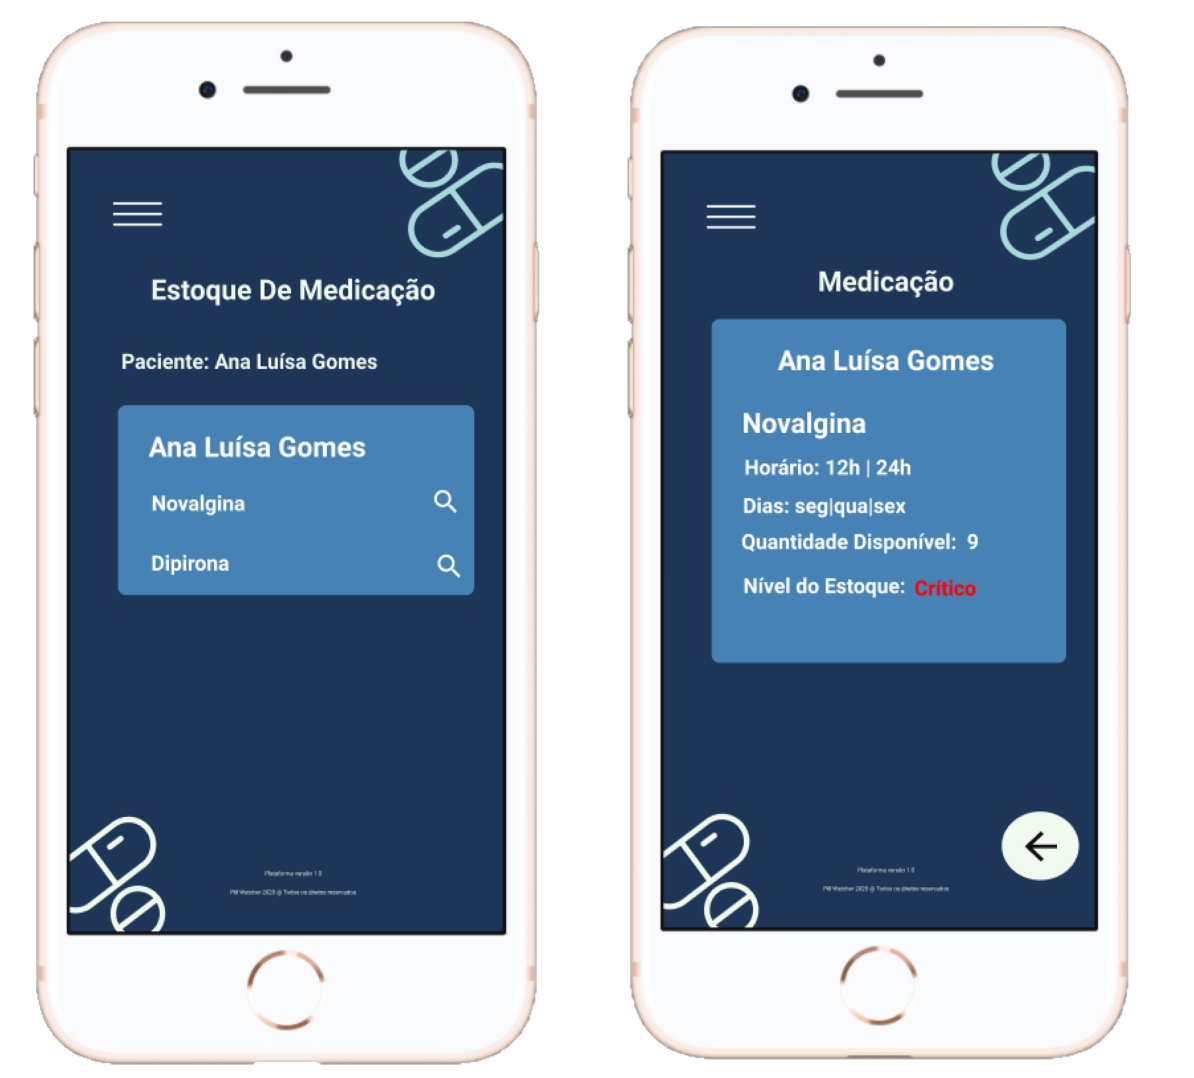
\includegraphics[width=8cm]{figuras/Software_Prototipo/Prototipo_Fluxo_Paciente_2.png}
    \label{fig:prototipo_paciente_fluxo_gerencia_estoque_pessoal}}
    \caption{Paciente - Parte 1}
\end{figure}

 

\begin{figure}[H]
    \centering
    \subfloat[][Relatório semanal de medicação]{
    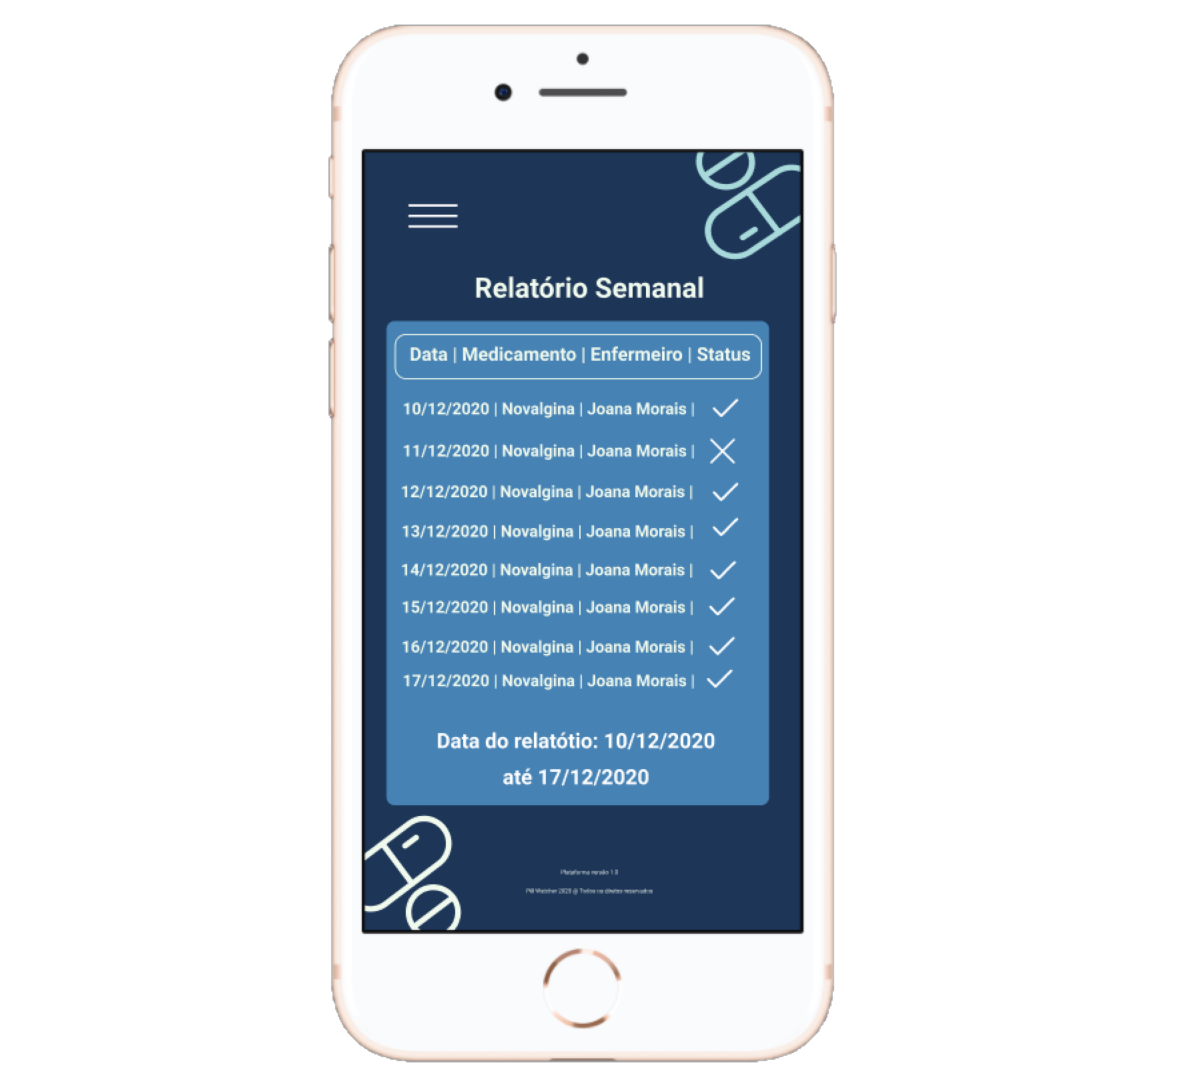
\includegraphics[width=8cm]{figuras/Software_Prototipo/Prototipo_Fluxo_Paciente_3.png}
    \label{fig:prototipo_paciente_relatorio_semanal}}
     \caption{Paciente - Parte 2}
\end{figure}

\ref{fig:prototipo_paciente_relatorio_semanal} expõe o relatório semanal de medicações de um paciente com a data, o nome do medicamento, o enfermeiro e o status.

